\documentclass[
%%%%% Styles and Sizes
%10pt,
%11pt,
%12pt,
fancyheadings, % headings with seplines and logo
%
%%%%% Printing, Color and Binding
%a4paper, 
%a5paper,
%twoside, % single sided printout
%oneside, % duplex printout (default)
%% binding correction is used to compensate for the paper lost during binding
%% of the document
%BCOR=0.7cm, % binding correction
%nobcorignoretitle, % do not ignore BCOR for title page
%% the following two options only concern the graphics included by the document
%% class
%grayscaletitle, % keep the title in grayscale
%grayscalebody, % keep the rest of the document in grayscale
%
%%%%% expert options: your mileage may vary
%baseclass=..., % special option to use a different document baseclass
]{stsreprt}

% Information for the Titlepage
\author{Fin Bießler}
\title{Randomized Generation of Flaky Test Suites}
\date{March 8, 2024}
\subject{Bachelor Thesis}
\professor{Prof. Dr. Sibylle Schupp}
\advisor{Daniel Rashedi}

\usepackage[utf8]{inputenc}
\usepackage{amsthm}
\usepackage{amsmath}
\usepackage{mathtools}
\usepackage{listings}
\usepackage{qtree}
\usepackage{verbatim}
\usepackage{longtable}
\usepackage[acronym]{glossaries}


\newtheorem{definition}{Definition}

\lstset{
    language=Python,
    basicstyle=\footnotesize,
    numbers=left,
    stepnumber=1,
    showstringspaces=false,
    tabsize=1,
    breaklines=true,
    breakatwhitespace=false,
    captionpos=b,
    xleftmargin=.0ex,
    frame=single,
}

\lstdefinelanguage{json}{
    basicstyle=\normalfont\ttfamily,
    numbers=left,
    numberstyle=\scriptsize,
    stepnumber=1,
    numbersep=8pt,
    showstringspaces=false,
    breaklines=true,
    frame=lines,
}


% Font and Fontencoding Magic
% FAQ: 
% http://tex.stackexchange.com/questions/664/why-should-i-use-usepackaget1fontenc
% http://en.wikipedia.org/wiki/Computer_Modern
% http://tex.stackexchange.com/questions/1390/latin-modern-vs-cm-super
\usepackage[T1]{fontenc}
\usepackage{lmodern}
\usepackage{hyperref}
%\usepackage{fix-cm}

% to generate some dummy text
\usepackage{lipsum}

\makeglossaries

\newacronym{apr}{APR}{Automatic Program Repair}
\newacronym{fl}{FL}{Fault Localization}
\newacronym{ast}{AST}{Abstract Syntax Tree}
\newacronym{json}{JSON}{JavaScript Object Notation}
\newacronym{sbfl}{SBFL}{Spectrum-Based Fault Localization}

\begin{document}
\frontmatter
\maketitle

\chapter*{Declaration of Originality\footnote{University of Tübingen, Department of Sociology}}

Hereby I confirm, Fin Bießler, Matr. Nr. 52906, that this assignment is
my own work and that I have only sought and used mentioned tools. \newline

\noindent I have clearly referenced in the text and the bibliography all sources used in the work
(printed sources, internet or any other source), including verbatim citations or paraphrases. \newline

\noindent I am aware of the fact that plagiarism is an attempt to deceit which, in case of recurrence, can result in a loss of test authorization. \newline

\noindent Furthermore, I confirm that neither this work nor parts of it have been previously, or
concurrently, used as an exam work – neither for other courses nor within other exam
processes.

\vspace*{4em}
\begin{tabular}[t]{c}
  Hamburg, March 8, 2024
\end{tabular}%
\hfill%
\begin{tabular}[t]{l}
  \rule{10em}{0.4pt}\\ Fin Bießler
\end{tabular}%
\hfill\strut

\chapter*{\centering \begin{normalsize}Abstract\end{normalsize}}
\begin{quotation}
 Automatic program repair and fault localization tools have been developed to aid developers while resolvinf software faults. State of the art tools extensively use test suite to find causes of errors, fix them and lastly validate their solution, but tests can be flaky in a sense that they do not behave deterministically, test might fail and succeed in independent test suite runs without altering source code. This is why flaky test are often removed from repair benchmarks testing such tools which limits the scope of such approaches. This is why this thesis aims at providing an approach that can randomly generate flaky test suites to aid the further development within the automatic program repair and fault localization research community. For this the program focuses on generating flaky test cases that are flaky due to randomness or test order dependency. As well as that we enabled the user of the program to configure the test suite generation such that parameters like test suite size, test suite composition or the failure chance of a flaky test could be determined. When evaluating we found that the program developed in that matter can actually generate flaky test suites with a majority of test cases that can be detected as flaky or faulty by the state of the art fault localization tool \texttt{CharmFL}. In further work the approach could be extended to cover more flakiness root causes.
\end{quotation}

\tableofcontents

\listoffigures{}

\lstlistoflistings

\listoftables

\printglossary[type=\acronymtype]

\mainmatter



\chapter{Introduction}
% \begin{itemize}
%     \item Domain
%     \item Problem description
%     \item Main approach/contribution
%     \item Evaluation results
%     \item (Related work)
%     \item Outline
% \end{itemize}
Software bugs play a huge role in the development and maintenance of software projects, they can be very expensive to fix and if not fixed they can have catastrophic impacts on the software system. 
This emphasizes the fact that software failures have to be dealt with and need to be fixed as soon as possible upon discovering them. \par
When a software malfunction is discovered the cause of it is often not obvious initially, developers have to investigate the cause and among others, dig through huge code bases, analyze log files and debug the code. 
All of this is very tedious and poses additional resource demand upon the company effectively resulting into increased costs. 
This is why \acrlong{apr} and \acrlong{fl} tools have been developed, to aid developers in the process of troubleshooting. 
On the one hand side \acrshort{apr} tools such as \texttt{SemFix} \cite{semfix:2013}, \texttt{Nopol} \cite{nopol:2017} or \texttt{Autofix} \cite{autofix:2014} aim at automatically locating software bugs and fixing them with minimal human intervention, reducing developer resources that have to be invested into software maintenance.
On the other hand side \acrshort{fl} tools such as \texttt{CharmFL} \cite{charmfl:2021} go a step back and just aid the developer in finding the faulty location in the first place. 
For this statements, methods/functions and classes are ranked by their suspiciousness, indicating the likelihood for them to be faulty.  \par
For both approaches, the state of the art tools utilize test suites to achieve this. 
Test suite outcomes are used as oracles to identify faulty locations within the code base, the problem with this is that test cases might not be deterministic.
Non-deterministic test cases are called flaky, their verdict changes between runs even though neither the tested code nor the test code itself is altered. 
Problematically flaky tests are often eradicated from benchmarks that test the previously mentioned tools, this obviously poses a threat to validity of such tools. It also reduces the confidence in these tools that they can be used to fix or identify faults in real world 
software project. \par

We contribute an approach for the generation of randomized flaky test suites to test the previously mentioned \acrshort{apr} and \acrshort{fl} tools on flaky test and evaluate their performance among these. 
The contribution includes the following key features:
\begin{itemize}
    \item Randomly generating flaky test suites stemming from test order dependency and randomness
    \item Providing different configurability options for the user of the tool, such as determining the total test number to be generated, the distribution of the number of test cases among the different flakiness categories and the probability with which a test case from the randomness category fails. 
    \item Sharing experimental evaluation results regarding the following two research questions:
    \begin{itemize}
        \item Are the generated test cases actually flaky?
        \item Does \texttt{CharmFL} detect the test cases to flaky or faulty?
    \end{itemize}
\end{itemize} \par
The evaluation has shown that the test cases generated are actually flaky with some minor exception for test cases that were intended to be non-flaky. 
Additionally, is \texttt{CharmFL} able to detect the flakiness and faultiness of test cases stemming from the randomness root cause where as the tool had a hard time to detect the flakiness caused by test order dependency. \par

The work is structured as follows. 
First, in Chapter \ref{ch:rel_work} related work regarding the presented approach is briefly presented. 
Second, in Chapter \ref{ch:background} theoretical concepts and definitions needed for the following discussions are introduced. 
Following that, in Chapter \ref{ch:approach} the main contribution on how to generate randomized flaky test suites is discussed. 
Furthermore, in Chapter \ref{ch:imple} some important aspects regarding the implementation of the tool are shared to the reader. 
Moreover, in Chapter \ref{ch:eval} results for the evaluation of the previously discussed approach are presented.
The thesis closes with Chapter \ref{ch:conc-futher-work}, where conclusions regarding the discussions are drawn as well as further work that is worth while doing is mentioned. 


\chapter{Related Work}\label{ch:rel_work}
In the following chapter insights on related work will be given. 
First, \acrlong{apr} and \acrlong{fl} techniques will be discussed. 
Second,  given the knowledge on prior approaches to generate flaky test suites key differences between these and the presented one will be highlighted. 
The relation of these techniques regarding the approach presented in this work is that the presented approach aims at improving existing \acrshort{apr} and \acrshort{fl} tools. 
This is done by providing flaky test suites to \acrshort{apr} and \acrshort{fl} tool developers such that they can extend their work to also repair faults in software projects that contain flaky test in their test suite. 

\section{Fault Localization Techniques}
According to Wong et al. \cite{fault-loc-survey:2016} \acrshort{fl} techniques can be categorized into two categories namely \textit{traditional \acrshort{fl} techniques} and \textit{advanced \acrshort{fl} techniques}. 
As mentioned previously \acrshort{fl} techniques are relevant for the presented work since the novel approach developed in this work aims at providing support to improve existing \acrshort{fl} techniques. 
In the subsequent section, a brief overview on these \acrshort{fl} techniques will be given. 
\subsubsection{Traditional Fault Localization Techniques}
These kind of techniques are traditional, basic and intuitive ways to locate faults in software. Even though they are not related to any recently developed \acrshort{fl} techniques we will nevertheless briefly state them for completeness purposes. They also represent the tedious work developers would have to perform when no \acrshort{fl} tools would be available to them. 
\begin{itemize}
    \item \textbf{Program Logging}: By adding amongst others \texttt{print} statements to the code base, program logs can be constructed that are used to identify faulty sections of the program 
    \item \textbf{Assertions}: Constraints are added to the programs source code that make the execution terminate if evaluated to false. 
    Like this erroneous behaviour can be identified during runtime.
    \item \textbf{Breakpoints}: The execution of a program halts at breakpoints where developers can inspect the state of the program at that point of the execution and alter it. 
    After the breakpoint, execution can be resumed to examine the progression of the respective bug.
    \item \textbf{Profiling}: Program metrics such as execution speed and memory usage are observed to optimize a program at most times. 
    Nevertheless it can be used to identify suspicious behaviour by for example detecting unexpected execution frequencies of different functions. 
\end{itemize}
\subsubsection{Advanced Fault Localization Techniques}
Due to the large size and scale of today's software projects the previously described traditional \acrshort{fl} techniques are not the most effective ways to identify the location of bug within source code, as they include a lot of manual work to be conducted. 
Thus different advanced approaches have have been developed, that address this problem in different manners. 
Some of the mayor approaches will be presented briefly in the following.
\begin{itemize}
    \item \textbf{Slice-Based Techniques}: The idea is to reduce the search space in which developers look for the cause of a bug within the source code by deleting unconcerned parts of the program with respect to a certain specification. 
    \textit{Static slicing} was fist proposed by Weiser in 1979, one of the main applications of static slicing \cite{slicing:1984} is to reduce the search space.
    The idea is that if a test case fails because of an incorrect variable value at a statement, then the fault should be found in the static slice of that variable-statement pair which then allows to reduce the search to that slice rather than the entire program. 
    \item \textbf{Program Spectrum-Based Techniques}: They use probabilistic- and statistical-based causality models in which information about execution behaviour is retrieved to identify buggy locations. For example code parts are ranked for suspiciousness according to how many failing or passing test cases executed them.\par
    Program spectra detail the execution information of a program. 
    These can be used to track a programs behaviour and thus localize faults. 
    Information on failing and passing test cases, and emphasising the contrast between them, can be used to identify suspicious code that is responsible for the fault. For this code coverage or Executable Statement Hit Spectrum (ESHS) indicate which parts of the program have been executed during the test run. 
    This information helps in narrowing down the search for the faulty component. \par
    In Chapter \ref{ch:eval} we will evaluate the newly developed approach in this work, by using the existing spectrum-based \acrshort{fl} tool \texttt{CharmFL} to identify flaky or faulty locations in the generated test cases. Since \texttt{CharmFL} uses a spectrum-based approach it is relevant to discuss this method in more detail in the following. \par 
    As proposed by Renieres and Reiss \cite{nearest-neighbour-program-spectra:2003} nearest-neighbor techniques contrast a failed test with a successful test that is most similar to the failed one in terms of distance between them. 
    A statement seems more \textit{suspicious} when it's execution pattern is closer to the failure pattern of all tests because it's more likely to be fault in this case.
    Likewise the farther a execution pattern is to the failing pattern the less likely it is to be faulty and thus it seems less \textit{suspicious}. Similarity-coefficients are used to measure and quantify the distance between statements. \par
    \textbf{Notation}
    \begin{itemize}
        \item $p$: a program
        \item $N_{CF}$: number of failed test cases that cover a statement
        \item $N_{UF}$: number of failed test cases that do not cover a statement
        \item $N_{CS}$: number of successful test cases that cover a statement
        \item $N_{US}$: number of successful test cases that do not cover a statement
        \item $N_{C}$:  total number of test cases that cover a statement
        \item $N_{U}$:  total number of test cases that do not cover a statement
        \item $N_{S}$:  total number of successful test cases
        \item $N_{F}$:  total number of failed test cases
        \item $t_{i}$: the ith test case
    \end{itemize}
    Among these similarity-coefficient based techniques is Tarantula \cite{tarantula:2002} a standard similarity-coefficient based metric that is used by \texttt{CharmFL}, for which the suspiciousness of a statement is calculated as 
    \[
        Suspiciousness(Tarantula) = \frac{\frac{N_{CF}}{N_F}}{\frac{N_{CF}}{N_F}+\frac{N_{CS}}{N_S}}.
    \]
    Another similarity coefficient that can be used when using \texttt{CharmFL} is Ochiai \cite{sim-coef-eval:2006} that is calculated as follows
    \[
        Suspiciousness(Ochiai) = \frac{N_{CF}}{\sqrt{N_F \times (N_{CF}+N_{CS})}}
    \]
    \item \textbf{Program State-Based Techniques}: The program state (programs variables and their respective values) is compared to some reference state during execution, this is also called relative debugging. 
    During runtime the current program state is compared to a reference state where the bug was not present to draw conclusions on the loction of the fault in the source code. 
    Another approach would be to modify the values of certain values to determine which cause the faulty execution. \par
    Regarding this Zeller and Hildebrandt proposed a technique called delta-debugging \cite{delta-debugging:2002}. Delta debugging compares program states between executions of failed and successful test cases via their memory graph. 
    Suspiciousness is determined by replacing variable values form successful tests with the ones from the same point of failed tests, afterwards execution is continued. 
    When the same error is observerd the location is still considered suspicious, otherwise not. 
    \item \textbf{Machine Learning-Based Techniques}: Based on machine learning algorithms it's tried to learn or deduce the location of a bug within a program.
    This is done based on input data such as statement coverage and the execution result of the test cases. \par
    % darf ich das einfach so aus einem anderen paper kopieren?
    A \acrshort{fl} techniques based on back-propagation networks that was proposed by Wong and Qi \cite{bp-fl:2009}, collects coverage data of each test case and the corresponding execution result, and they are used together to train a BP neural network so that the network can learn the relationship between them. 
    Then, the coverage of a suite of virtual test cases that each covers only one statement in the program is input to the trained BP network, and the outputs can be regarded as the likelihood of each statement containing the bug.
\end{itemize}
\section{Automatic Program Repair}
Software maintenance is costly and drains many resources such as money and time, thus as the name suggests, \acrshort{apr} aims at finding faults in software and provide fixes for these, so called \textit{patches}. 
Test suites play a significant role in such techniques as they function as executable software specifications. 
Test suite based repair was initially introduced by GenProg \cite{genprog:2012}, an \acrshort{apr} system that is based on genetic programming.
Research has developed and new \acrshort{apr} approaches were discovered. These approaches can be divided into two categories.
First, generate-and-validate techniques and second synthesis-based techniques. 
In the following a brief overview of both approaches will be given.
\subsubsection{Generate-and-Validate Approaches}
Generate-and-validate approaches like Astor \cite{astor:2019}, CapGen \cite{capgen:2018} or the previously mentioned GenProg method all fall into this category. 
The key characteristic of this approach is to first generate as many patches fixing the viewed bug. 
Second, the test-suite is used to validate whether there is a patch among the candidates that makes all test cases pass. 
\subsubsection{Synthesis-Based Approaches}
On the other hand synthesis-based approaches such as SemFix \cite{semfix:2013}, Nopol \cite{nopol:2017} or Autofix \cite{autofix:2014} address the problem in a reversed manner. 
They first execute the test-suite and extract constraints from the execution results, based on which a patch is synthesized by using a constraint solver. \cite{apr-benchmark-quixbugs:2021} \par
A problem that arises for these techniques is that flaky tests are often removed from the benchmarks implementing these techniques \cite{flaky-impact-repair:2021}.
Though flaky tests are prevalent in real world software projects, thus the absence of testing these tools on flaky test might pose a threat to validity to them. 
\section{Generation of Test-Suites}\label{sec:prev_approach}
Now that a brief overview on \acrshort{apr} and \acrshort{fl} techniques were given, it's going to be continued with giving a brief introduction into previous approaches to generate flaky test suites.\par
Regarding Gruber et. al. \cite{empirical-flaky:2021} the two state of the art techniques on generating flaky test suites were more of a passive fashion, in the sense that no new code was generated ab initio. 
Rather existing code was collected and shipped as a dataset for flaky test suites. \par
For this two major approaches are known to the community. 
First, looking for commits in version control systems or bug trackers that fixed issues related to flakiness. 
Second, collect tests from existing software projects and rerun them a certain number of times and determine whether their verdicts change through out the executing when not changing the code. 
Tests that had passing runs as well as failing runs are then coined as flaky and are collected into the dataset of flaky test suites.  \par
So to emphasize the difference between existing approaches on generating flaky test suites and the one presented in this thesis, recall that previously existing code was passively collected where as in the presented novel approach new code is actively randomly generated ab initio. 
\chapter{Theoretical Background}\label{ch:background}
This section covers necessary definitions and terms needed for the subsequent chapters of this thesis. 

\section{Test-Cases and Test-Suites}
Because we present an approach to generate randomized test suites in this thesis, the following section first defines what test-cases are, how they are combined into test-suites and what purpose they serve in a real-life software project.

\subsubsection{Test-Cases}
A test-case is piece of software that is written to test parts of the production code of their respective software project. According to the widely used \textit{Arrange Act Assert} (AAA) pattern a test-case can be divided up into three sections \cite{darbord:2023}. In the following this pattern is going to be formalized and further described. \par
\begin{itemize}
    \item $n$: Number of statements in the test
    \item $s_n$: Set of statements in the test
    \item $s_i$: Statement $i$ of the test
    \item $s_i \forall i \in [1, .., k]$: Arrange statements of the test
    \item $s_i \forall i \in [k+1, .., l]$: Act statements of the test
    \item $s_i \forall i \in [l+1, .., n]$: Assert statements of the test
\end{itemize} 
Now a brief description for each individual statements section is going to follow.\par
\textbf{The $k$ arrange statements:} For testing the production code several prerequisites have to be prepared such as setting up the objects to be tested for instance different variables have to be assigned. Furthermore 
some dependencies might have to be mocked because they are not tested in the concerned test-case but are needed for the piece of code that is being tested. \par
\textbf{The $l-k$ act statements:} In this section the actual functionality that is going to be tested is carried out and the respective actual result is saved in some manner to later check it's validity. This can be just one simple functionality or a more complex one that is composed from many simple ones. \par
\textbf{The $n-l-k$ assert statements:} In this last section the result is verified by asserting that the obtained actual result from the second section is equal to some expected result that is defined beforehand. \par
An example of a simple function and its respective test-case is given in Listing \ref{lst:simple_test}. 
In lines one and two the function to be tested is defined. 
Following that in  lines four to eleven the corresponding test is defined.
Furthermore in lines five to seven the needed variables are \textit{arranged}, additionally in line nine the actual value is produced by calling the function to be tested, which corresponds to the \textit{act} section described above. 
Lastly in line eleven the actual and expected values are \textit{asserted} to be equal. 

\subsubsection{Test-Suites}
Test-suites are collections of several test-cases that depict the functionality of the tested software. They are used to ensure that production code is working as intended by the developer. When new production code is deployed test-suites can be carried out to check whether the newly deployed code did break existing functionality, this method is called regression testing. Sizes of test-suites depend on the size of the software project that is tested by the test-suite, so they can vary from just a few test cases to an accumulation of many test-cases.

\begin{lstlisting}[language=Python, caption={A simple function and it's respecive test-case }, label=lst:simple_test]
    def add(a, b):
        return a + b

    def test_add():
        a = 2
        b = 2
        expected = 4

        actual = add(a, b)

        assert actual == expected
\end{lstlisting}

\section{Flaky Tests}
The term "flaky" means "unreliable", when a test is depicted as flaky it means that this tests outcome is not reliable and can pass and fail for the same software version, when run multiple times. 
Following Luo et al. \cite{luo:2014} the tests are non-deterministic with respect to a given software version. 
This creates problems when trying to automatically locate software faults and later on resolve those faults. \par

Luo et al. \cite{luo:2014} have stated that flakiness in test-suites always stems from one of 10 root causes. 
In the following subsections, the flakiness categories relevant for the approach presented in Chapter \ref{ch:approach} will be described. 
In additions to that theoretical terms will be defined. 

\section{Flaky Tests Due to Randomness}
As described by Luo et al. \cite{luo:2014} the use of random numbers can make tests flaky. When using random number generators flakiness manifests when not handling all possible numbers that can be generated including all edge cases. For example, a certain test fails when an one-bit random number is generated to zero, because the tests only handles the cases where it's one and undefined behaviour occurs when the generated number is zero resulting in the respective test to fail. 

\section{Flaky Tests Due to Test Order Dependency}\label{sec:theory_order_dep}
First of all test order-dependent tests are tests where the outcome depends on the order in which the tests are run. 
Generally tests should be written in an isolated way resulting in independence between them and enabling any execution order to succeed. 
But in reality this is not always the case. This behaviour occurs when tests work on a shared state that is not properly setup or cleaned. 
This state can either be in main memory (\textit{global} variables in Python) or some external resources like \textit{files} or \textit{databases}. 
On the one hand a "polluter" test was run before another test which fails the latter test because it expects to find the state to be as initialized, but the first test altered this state. 
Or on the other hand "state-setting" test was not run before another test that expects a preceding test to prepare the state in a certain way to pass. \par 
Definitions proposed by Shi et. al. \cite{ifixflakies:2019} concerning test order-dependent tests, that we use to describe the approach on how to randomly generate test-cases from that category, will be given in the following. 


\begin{itemize}
\item Let $T$ be the set of all tests in the test suite.
\item A \textit{test order} is a sequence of a subset of tests from $T$.
\item For a test order $O$ that has a test $t \in T$, let $run_{t}(O)$ be the result of the test $t$ when run in the test order $O$.
\item $run(O)$ is the result of the last test run in order $O$.
\item $[t]$ is the test order consisting of just one test $t$.
\item $O + O^{'}$ is the concatenation of two test orders $O$ and $O^{'}$. 
\end{itemize}

\begin{definition}
    A test $t \in T$ has a \textbf{passing test order} or a \textbf{failing test order} $O$ if $run_t(O) = PASS$ or $run_t(O) = FAIL$, respectively.
\end{definition}

\begin{definition}
    An \textbf{order-dependent test} $t \in T$ has a passing test order $O$ and a failing test order $O^{'} \neq O$
\end{definition}

Order-dependent tests can be classified into two categories, \textit{victim} and \textit{polluter}. Furthermore, other tests that are related to test-order-dependent test but are not flaky themselves can be classified into the following three categories: \textit{cleaner}, \textit{brittle} and \textit{state-setter}. In the following, these categories will be defined. 

\begin{definition}[Victim]
    An order-dependent test $v \in T$ is a \textbf{victim} if $run([v]) = PASS$
\end{definition} 

\begin{definition}[Polluter]
    A test order (with one or more tests) P is a \textbf{polluter} for a victim $v$ if $run(P + [v]) = FAIL$
\end{definition}

\begin{definition}[Cleaner]
    A test order (with one or more tests) C is a \textbf{cleaner} for a polluter $P$ and its victim $v$ if $run(P + C + [v]) = PASS$
\end{definition}

\begin{definition}[Brittle]
    An order-dependent test $b \in T$ is a \textbf{brittle} if $run([b]) = FAIL$
\end{definition}

\begin{definition}[State-Setter] %TODO: Schreibweise?
    A test order S is a \textbf{state-setter} for a brittle if $run(S + [b]) = PASS$
\end{definition}
% Quelle: https://dl.acm.org/doi/pdf/10.1145/3338906.3338925

\section{Abstract Syntax Tree}
There are two reasons for generating the randomized test-suites on the \acrlong{ast} level. 
First, to avoid directly working with source code strings. 
Second, to conveniently transform them to source code and write them to their respective files in the file system. 
Thus a brief introduction to the \acrshort{ast} is given in the following. \par

An \acrshort{ast} is a tree representation of source code that contains the programs constructs such as if-statements, loops, or variable assignments as it's nodes the edges between this nodes indicate the relation between the programs constructs. 
For example, all statements that are carried out within a loop are children of the loop node in the tree. 
Depending of the implementation of the represented programming language, the tree can carry additional information such as the source code lines in which the respective nodes are written in. 
Conveniently each node and it's children forms new subtree that is also an \acrshort{ast}, which makes traversing the tree recursively and interchanging parts of the structure very natural.\par

In Figure \ref{fig:simple_ast} the \acrshort{ast} for the expression \lstinline{a=a+1} is shown. 
The \textit{root node} is a variable assignment where the right child is the source, in this case a addition binary operation with the operands variable \textit{a} and constant $1$. 
The left child of the variable assignment node is the target to which the result of the operation should be assigned to, in this case the variable \textit{a}.

\begin{figure}[h]
    \centering
    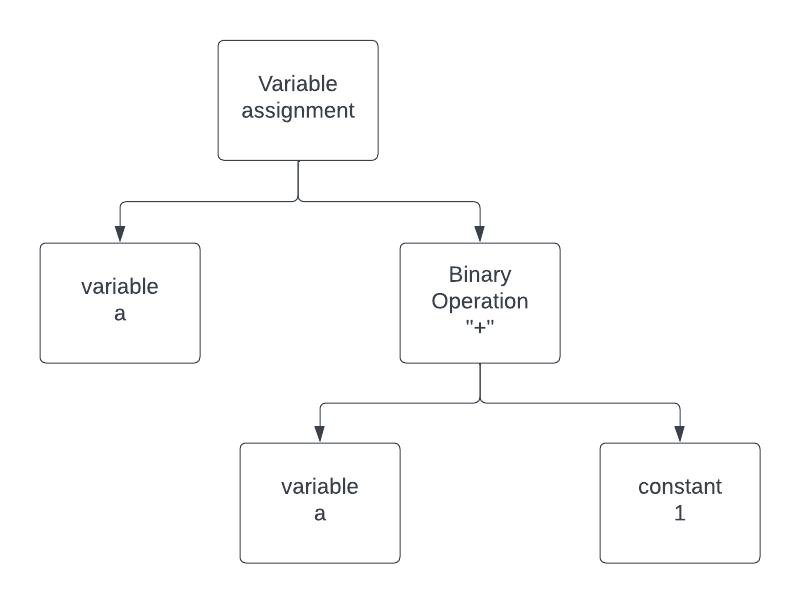
\includegraphics[width=0.5\textwidth]{img/simple_ast.png}
    \caption{AST of the expression  \lstinline{a=a+1}}
    \label{fig:simple_ast}
\end{figure}


\chapter{Generating Randomized Test-Suites} \label{ch:approach}
In the following chapter the novel approach to generate randomized test-suites is going to be presented. In contrast to the approach presented in Section \ref{sec:prev_approach}, the novel approach actively generates new test cases and respective functions ab initio, rather than passively collecting them from existing software repositories or bug tracking systems. \par
\section{Generators}
Regarding Luo et. al. \cite{luo:2014} flakiness stems from one of ten following flakiness categories: \textit{async wait}, \textit{concurrency}, \textit{test order dependency}, \textit{resource leak}, \textit{network}, \textit{time}, \textit{I/O}, \textit{randomness}, \textit{floating point operations} and \textit{unordered collections}.
One can develop approaches for each category and then combine them and generate test suites containing tests that are flaky with regard to the implemented categories. 
Depending on the flakiness category different approaches have to be followed. 
For this generators for all considered categories in this thesis are implemented. 
In the following subsections all regarded flakiness root causes and their respective generators are presented. 

\subsection{Randomness}\label{sec:rand}
The randomness root cause is the first one to be considered.
We decided to cover this flakiness category to provide a simple start to initialize the work on this approach. 
In the following subsection the approach on how to implement generators for this root cause is going to be presented. 
The key idea is to generate arithmetical expressions of random length composed of random operands and operators which are than randomly interfered by some noise value. 
To elaborate this in more detail the following is defined: 
\begin{itemize}
    \item $(o_k)_{k \in [1, ..., n]}$: Sequence of $n$ random operators
    \item $(v_{k})_{k \in [1, ..., n+1]}$: Sequence of $n+1$ random numbers as operands 
    \item $X$: Random variable that represents the noise interference subexpression, consisting of an operator $o_X$ and a value $v_X$, that can be defined as
    \begin{itemize}
        \item $P(X=+0)=0.7$, here $o_X = +$ and $v_X = 0$
        \item $P(X=+1)=0.3$, here $o_X = +$ and $v_X = 1$
    \end{itemize}
\end{itemize} 

using the above symbols the previously discussed arithmetical expressions can be defined like the following:
\[
    v_1 o_1 v_2 \cdots  v_n o_n v_{n+1} X = v_1 o_1 v_2 \cdots  v_n o_n v_{n+1} o_X v_X
\]
\subsubsection{Example}
Let 
\begin{gather*}
    (v_{k})_{k \in [1, ..., n+1]} = (+,-,\cdot, \%) \\
    (o_k)_{k \in [1, ..., n]} = (2,2,3,4,5) \\
\end{gather*}
Then with a probability of $0.7$ the arithmetical expression equals
\[
    \dfrac{(2 + 2 - 3) \cdot 4 }{5} + 0
\]
and with a probability of $0.3$ it equals 
\[
    \dfrac{(2 + 2 - 3) \cdot 4 }{5} + 1.
\]
For the randomization subexpression one can differentiate two cases, either the arithmetical expression is interfered with the noise or it is left untouched.
Considering the first case, there are five operator and operand combinations that have to be excluded, namely division and zero as it would result in an undefined operation, subtraction or addition paired with the operand zero and multiplication or division with the operand one, as these are the neutral operations for the respective operands and would lead into not interfering the arithmetical expression at all. \par 
Considering the second case, we also have to exclude the operator and operand combination division and zero as it would again result in an undefined operation. 
In contrast to the first case, the goal is to not interfere the arithmetical expression with the interference noise subexpression, thus the previously excluded combinations are the only ones that are allowed. 
Namely subtraction or addition operators with zero as the operand and division or multiplication operators with one as the operand. 

\subsection{Test Order Dependency}
For the second root cause that is examined in this thesis one can use the patterns discussed in Section \ref{sec:theory_order_dep}, namely victim and polluter along side with brittle and state-setter.
In the following section we will formalize an approach on how to randomly generate flaky tests based on these patterns. \par

First one can define the concatenation of two sequences as the following.
\begin{definition}[Sequence Concatenation]
    Let $(a_n)_{n \in \mathbb{N}}$ and $(b_k)_{k \in \mathbb{N}}$, then
    \[
       (a_n) + (b_n) \coloneqq (a_1, a_2, \cdots , a_n, b_1, b_2, \cdots b_k)
    \]
\end{definition}
\subsubsection{Victim- and Polluter-Pattern}
For this pattern a global state has to be defined, that is then used by the polluter and victim test cases. 
Therefore we have to look at the generated test cases in an accumulated fashion, in the following we call these concatenated test cases a test case module. \par
This test case module $T$ consists of multiple parts defined in the following sequences:
\begin{itemize}
    \item $(g_n)_{n \in \mathbb{N}}$: Sequence containing all statements related to the initialization of the global state used by the victim and polluter test cases
    \item $(v_k)_{k \in \mathbb{N}}$: Sequence containing multiple test case definitions that function as victims regarding the global state
    \item $(p_l)_{l \in \mathbb{N}}$: Sequence containing the polluter test case definition regarding the global state
\end{itemize}
Using the previously described sequences we can define the test case module as the concatenation of them
\[
    T = g_n + v_k + p_l 
\]
It is important that the state initialization statements contained in set $g_n$ are carried out before the victim and polluter test cases contained in sets $v_k$ and $p_l$, since the global state variables initialized in $g_n$ are used in the test cases contained in $v_k$ and $p_l$. \par
The victim test cases assert that the global state contains a success state and thus only pass if this is the case, in contrast the polluter test case firstly \textit{pollutes} the global state by altering it to contain a failure state and then secondly asserts the global state to contain the failure state. 
For the victim- and polluter pattern the global state is initialized with a success state, this leads to the fact that the polluter test case always succeeds and the victim test cases only succeed when they are run prior to the polluter. \par
We consider the previously discussed test cases to be a sequence of the form
\[
    t_1, t_2, \cdots, t_{n-1}, t_n.
\]
Where $t_i$ is the i-th test case in the sequence. Now let $t_p$ be the polluter test case within the sequence, then the following holds
\begin{equation*}
\forall i,p \in [1, ..., n]:
t_i=
    \begin{cases}
        PASS  & if \; i \leq p  \\
        FAIL  & if \; i > p .
    \end{cases}
\end{equation*}
\subsubsection{Brittle- and State-Setter-Pattern}
As well as for the victim- and polluter-pattern a global state has to be defined for the brittle- and state-setter-pattern. 
For the brittle- and state-setter-pattern the generated test cases concatenated together also form a test case module. 
The module can be defined as the concatenation of the following sequences:
\begin{itemize}
    \item $(g_n)_{n \in \mathbb{N}}$: Sequence containing all statements related to the initialization of the global state used by the brittle and state-setter test cases
    \item $(b_k)_{k \in \mathbb{N}}$: Sequence containing multiple test case definitions that function as brittles regarding the global state
    \item $(s_l)_{l \in \mathbb{N}}$: Sequence containing the state-setter test case definition regarding the global state
\end{itemize}

Using the previously described sequences the test case module yields 
\[
    T = g_n + b_n + s_n 
\]
The $+$-operator has the same notion as in the previous section. The main difference to the victim- and polluter-pattern is that the state is initially set to a failure state rather than a success state. The brittle asserts that the global state contains a success state in the same fashion as the victim previously. The state-setter in contrast to the polluter sets the global state to a success state rather than to failure state. This leads to the fact that the state-setter test case always succeeds and the brittle test cases only succeed when the state-setter test case was run prior to them. \par
To formalize this a bit further again assume the test cases to be a sequence of the form
\[
    t_1, t_2, \cdots, t_{n-1}, t_n.
\]
Where $t_i$ is the i-th test case in the sequence. Now let $t_s$ be the state-setter test case within the sequence, then the following holds
\begin{equation*}
\forall i,s \in [1, ..., n]:
t_i=
    \begin{cases}
        FAIL  & if \; i \leq s  \\ 
        PASS  & if \; i > s.
    \end{cases}
\end{equation*}
Thus when executing the test cases described in the previous approaches in random order the test will be flaky. 
Note that even though the tests are executed in random order this does not fall into the randomness flakiness category, since order dependencies within the tests are the actual root cause of the flakiness. 
One can emphasize this by considering random order execution of order-independent tests, which in turn would be non-flaky assuming that they are non-flaky internally. \par
Concluding this, the theoretical approach on how to generate the test cases was elaborated. 
In the following section elaborates how to further randomize the generation. 
With this, one tries to ensure that the generated test cases within one flakiness category differ from each other. 
After that implementation details will be given in Chapter \ref{ch:imple}, problems that occurred and decisions that were made will be discussed. \par

In the following sections additional measures to randomize the generation will be discussed. 
For the two approaches covered in the previous sections the one concerning randomness is already inherently randomized due to the random arithmetical expression. 
For the test order-dependent tests some steps have to be taken to randomize their generation, which will be elaborated in the subsequent sections. 

\section{Randomizing by Naming and Value Selection}
Considering the variable that holds the state that results in tests to be order-dependent, it is straightforward to randomize this by randomly picking the variable name. 
Furthermore the previously discussed success and failure states can be of any data type and value, since the actual value is irrelevant. 
The key relevance lies in a value being defined as a success state and all other values being a failure state.
For example the states data type could be \texttt{integer}, where the success state is the value \texttt{1} and all other integer values being failure states. 
Another example would be to define the states to be of \texttt{string} type, where the success state is the value \texttt{"success"} and the failure state is the value \texttt{"failure"}. \par
Thus the state might be of any data type and for each collection of order-dependent tests the success value can be defined independently leading to randomized tests. 
Moreover when the value of the failure state can be randomly picked from the data types range excluding the success value. 
\subsubsection{Example}
In the following two examples class definitions taken from a randomly generated test-suite are taken and showcased. 
These use the previously discussed randomization strategy. 
The state variable \texttt{member\_state\_m }is randomized by adding the random post-fix \texttt{m}, \texttt{member\_state\_n} and \texttt{n} vice versa. 
\begin{lstlisting}[language=Python, caption={Class definition used in a flaky test from the victim- and polluter-pattern}, label=lst:class_vic_pol]
class class_victim_polluter_0dac8877ef91402a9a80a3851b964588:
    member_state_m = 'success_state'

    def set_member_state_m(self, value):
        self.member_state_m = value

    def get_member_state_m(self):
        return self.member_state_m
\end{lstlisting}

\begin{lstlisting}[language=Python, caption={Class definition used in a flaky test from the brittle- and state-setter-pattern}, label=lst:class_brit_state_setter]
class class_brittle_state_setter_61030948535442d0b9d02d470eacf05f:
    member_state_n = 'failure_state'

    def set_member_state_n(self, value):
        self.member_state_n = value

    def get_member_state_n(self):
        return self.member_state_n

    def dummy_function(self):
        return 48
\end{lstlisting}
For Listing \ref{lst:class_vic_pol} the flakiness is obtained by performing multiple operations on the \newline \texttt{member\_state\_m} variable. 
In the polluter test case, the setter method of the class is used to alter the value of the state to contain a failure state.
Victim test cases use the getter method to assert that the \texttt{member\_state\_m} variable contains a success state. 
All victim test cases that are executed after the polluter test case fail.
The test cases are made flaky by randomizing the order in which they are executed. \par

For Listing \ref{lst:class_brit_state_setter} the flakiness is obtained by performing similar operations on the \texttt{member\_state\_n} variable. 
In the state-setter test case, the setter method of the class is used to alter the value of the state to contain a success state. 
In the brittle test cases the getter method of the class is used to assert that the state contains a success state. 
All brittle test cases that are executed before the state-setter test case fail. 
The test cases are made flaky by randomizing the order in which they are executed.

\section{Randomizing by Combining Flakiness Categories}\label{sec:rand_by_comb}
Within the randomness flakiness category different arithmetical expressions can be generated, for example expressions using all arithmetical operators or expression using just one operator. 
Following that, one can generate test cases that assert the outcome of multiple arithmetical expressions at once in contrast to only one at the time.
This allows for further randomization by combining different expression types and varying the number of expression results to be asserted. \par
Note that asserting multiple expression results within a test case that fail with some probability result in the whole test case to be more flaky. 
To describe that in more detail assume there is a test case $T$ with multiple assertions, then the following can be defined:
\begin{itemize}
    \item $n$: Number of assertions carried out within test case $T$
    \item $P_n$: Set of $n$ probabilities with which the respective assertions succeed
\end{itemize}
Then the overall flakiness probability of the whole test case yields 
\[
    (1 - p_1) \cdot (1-p_2) \cdot \cdots \cdot (1-p_{n-1}) \cdot (1-p_{n})
\]
with $p_i \in P_n$. \par
Note that the success probability of a assertion directly corresponds to the probability $p$ used in Section \ref{sec:rand}.


\section{Randomizing Test-Suite Composition}
Previously we discussed \textit{intra}-randomization techniques, in the sense that they randomized the generation of a single test case in particular. 
The following measures to be discussed are \textit{inter}-randomization techniques, in the sense that they randomize the generation of the whole test-suite. \par

\subsubsection{Test-Suite Size}
The number of test cases generated for the test-suite can also be randomized. 
Therefore a lower- and upper-bound for the test case number is being configured.
After that for each run of the test-suite generation a random number between the lower- and upper-bound is picked. 
That number then indicates how many test cases have to be generated in total for that generation run. 

\subsubsection{Flakiness Categories}
As discussed in previous sections the generation of test cases within the test-suite is split among the different flakiness categories stemming from the actual flakiness root causes. 
The two elaborated flakiness categories actually have a few sub-categories originating from different implementation approaches. 
This is why there are a number of different flakiness sub-categories from which a test-case could be generated, this offers more room for randomization which will be briefly discussed in the following. \par

For each flakiness sub-category a relative frequency is configured. 
When the generation for an individual sub-category starts, the relative frequency is then multiplied with the previously randomized total count of test cases contained in the test-suite to indicate how many test cases from the respective category should be generated. 
Since the total count of test-cases is random within a previously defined range, the number of test cases generated from an individual sub-category is random as well. 



\section{Randomizing by Adding Dummy Code}
Another way of randomizing the generation of the test suite is to add dummy code to the test files. 
This code does not contribute to the flakiness of the tests it rather adds diversity to the randomization. 
Random functions and methods are generated that are then called within the tests but their return values do not contribute to the tests assertions and thus do not effect the tests result when executing them. 
The actual behaviour of the dummy code can be very diverse, to name a few one could perform side effects such as printing to the standard output, calculate some random operation or return some static value. \par
Besides the added diversity of the generation, including dummy code brings another benefit.
It adds complexity to the generated test suite in the form of non-flaky methods which allows for better evaluation when using \acrshort{apr} or \acrshort{fl} tools on the test suite. 
There are not only flaky methods in the test suite that should be detected by the respective tools, like this there are also non-flaky methods that should not be detected by such tools.
Listing \ref{lst:class_brit_state_setter} shows a class that implements a dummy function that returns a static value, this function is then called in a test case of the generated test suite. 





\chapter{Implementation}\label{ch:imple}
In the following chapter implementation details on the theoretically presented approach will be given.
For that certain decisions that were made along the implementation process will be explained and discussed. 
First, the selection of the used testing framework will be discussed. 
Second, measurements to enable the configurability of the test suite generation will be presented.
After that the software architecture will be described briefly along with a presentation of a short code example. 
The chapter will close with a brief validation of the implementation, in the sense that the proposed configurability of the test suite generation works as intended. 



\section{Testing Framework}
Concerning the testing framework for which the test cases are randomly generated with the presented tool, there were two major options to chose from. 
One being \texttt{pytest} the other being \texttt{PyUnit}. In this case we decided to use \texttt{pytest} rather than \texttt{PyUnit} mainly due to it's simpler usage.
Less "boilerplate" code is needed for test cases in \texttt{pytest}, a test function must be inside a file that follows one of the following two file name patterns, \lstinline{test_*.py} or \lstinline{*_test.py} and the function itself must be prefixed with the word \lstinline{test} to be discovered. \par
Additionally, there are multiple packages for \texttt{pytest} that are handy while implementing the presented approach.
First, being \texttt{pytest-random-order} that allows for configuration of the test runs such that tests are run in a random order. 
Like this the test order-dependent test-case become flaky in the first place.
Second, \texttt{pytest-json-report} that simplified the evaluation of the research questions, because it puts out a \lstinline{.json} file that contains all information on the outcome of a test suite run after it was performed, allowing for analysis regarding the number of tests run or which tests passed or failed in which runs.
\section{Configurability of Test Suite Generation}
In the following section the configurability measurements that were taken when developing the presented tool will be presented. \par
Users of the tool can access it through the command line interface and give a path to a configuration file in \acrlong{json} format as an argument. 
When not providing this argument, the tool uses a predefined \lstinline{config.json} file that is contained in the project.
This \acrshort{json} file has the following structure and semantics. \par 
Listing \ref{lst:config} provides an example of such a config file.
First, it contains values for the maximum and minimum number of test cases generated, between these a random number then is chosen to define the number of test that should be generated in a generation run. \par
Second, for each flakiness category there will be a \acrshort{json} object always containing at least one value depicting the share of the total test case number to be from the respective flakiness category. \par
Additionally there can be flakiness category specific configuration values, for example the flakiness probability for randomness flakiness categories indicating the probability with which a test case form this category should be flaky.  

\begin{lstlisting}[language=json,firstnumber=1, caption={Examplary \lstinline{config.json} file}, label=lst:config]
{
  "max_total_test_count": 550,
  "min_total_test_count": 500,
  "random_api": {
    "summation": {
      "test_number_share": 0.1,
      "max_summation_depth":  50,
      "max_summand": 1000,
      "flakiness_prob":  0.5
    },
    "multiplication": {
      "test_number_share": 0.1,
      "max_multiplication_depth":  100,
      "max_multiplicand": 10,
      "flakiness_prob":  0.5
    },
    "arithmetical": {
      "test_number_share": 0.1,
      "max_expression_depth":  100,
      "flakiness_prob":  0.5
    },
  },
  "test_order_dependent": {
    "basic_victim_polluter": {
      "test_number_share": 0.1,
      "flakiness_prob":  0.5
    },
    "basic_brittle_state_setter": {
      "test_number_share": 0.1,
      "flakiness_prob":  0.5
    },
    "classes_brittle_state_setter": {
      "test_number_share": 0.1,
      "flakiness_prob":  0.5
    }
  }
}
\end{lstlisting}



\section{Software Architecture}
In the center of the implementation are generator classes for each flakiness category from which the test cases can stem from. 
These generator classes then generate test cases on the \acrshort{ast} level using the \texttt{ast} package.
The \texttt{ast} package provide the datastructures that are used to construct and generate the test cases. 
It contains classes for expressions, statements and function definitions for example. 
Following that the \acrshort{ast}s of the test cases are converted into source code using the \texttt{astor} package. 
The \texttt{astor} package supplies methods to convert the generated \acrshort{ast}s to source code. 
Finally the generated source code is then written to a file and persisted in this way.\par
Now one exemplary generator class and it's respective test case generation functions will be presented and explained.
The presented generator class implements the generation of test cases from the randomness category, to be more specific it generates flaky test suites that use random summation expressions that are then made flaky by adding some noise with a certain probability.
\begin{lstlisting}[language=Python, caption={Generator class from the randomness category}\label{lst:summ_generator}]
class SummationGenerator(RandomApiGenerator):
    def __init__(self, flakiness_prob):
        self.flakiness_prob = flakiness_prob

    # Generates function that adds a summand as often as summation_depth indicates and then adds a noise with some prob
    # like summation_depth=3, summand=5: 5 + 5 + 5 or 5 + 5 + 5 + 0.1
    def generate_flaky_function_tree(
        self, 
        summation_depth, 
        function_identifier
    ):
        epsilon = ast.Constant(0.1)
        zero = ast.Constant(0)
        statements = []
        result = ast.Name('result')

        if_expr = ast.IfExp(
            self.generate_compare_lt_expression(
            self.generate_random_float_number_expression(), ast.Constant(self.flakiness_prob)),
            zero,
            epsilon
        )

        summation_expression = ast.Expression(
            ast.BinOp(left=ast.Name(id='summand'), 
            op=ast.Add(), 
            right=if_expr)
        )
        assignment = ast.Assign([result], summation_expression)
        statements.append(assignment)

        for i in range(summation_depth-1):
            summation_expression = \
                ast.Expression(
                    ast.BinOp(left=ast.Name(id='summand'),
                    op=ast.Add(), 
                    right=result)
                )
            assignment = ast.Assign([result], summation_expression)
            statements.append(assignment)

        statements.append(ast.Return(result))

        return ast.FunctionDef(
            'flaky_summation_' + function_identifier,
            ast.arguments([], [ast.arg(arg='summand')], defaults=[]),
            statements,
            []
        )

    # Generates one line function that asserts equality between the call of the flaky function and non-flaky summation
    def generate_test_tree(
        self, summand, 
        summation_depth, 
        function_identifier
    ):
        actual = ast.Name('actual')
        expected = ast.Name('expected')
        actual_value = ast.Call(
            func=ast.Name('random_api_summation.flaky_summation_' + function_identifier), 
            args=[ast.Constant(summand)], keywords=[]
        )

        statements = [
            ast.Assign(
                targets=[actual], 
                value=actual_value,
                type_ignores=[]
            ),
            ast.Assign(
                targets=[expected], 
                value=ast.Constant(summation_depth * summand),
                type_ignores=[]
            ),
        ]

        random.shuffle(statements)

        statements.append(
            self.generate_assert_equality_expression(expected, actual)
        )

        test_function = ast.FunctionDef(
            'test_sum_' + function_identifier,
            ast.arguments([], [], defaults=[]),
            statements,
            []
        )
        return test_function

\end{lstlisting}
Note that there are two methods implemented in this class one for generating the flaky test case and the other for generating the function that makes the test case flaky. 
We will first cover the function \lstinline{generate_flaky_function_tree}. \par
First, in lines 12 to 15 variables holding \texttt{Constant} and \texttt{Name} \acrshort{ast} nodes and an array for holding the functions statements are initialized. 
Second, in lines 17 to 22 a ternary conditional expression that yields the previously generated \texttt{epsilon} with some flakiness probability, given as a parameter of the method, otherwise zero is generated. 
Following that in lines 24 to 42  summation expressions of length \lstinline{summation_depth} are generated and appended to the statement array. 
As well as that a return statement returning the result of the previous additions is appended. 
In conclusion a function definition containing the previously generated statements is generated. \par
Now we will discuss the generation of the test case itself, that uses the previously generated flaky function.
First, in lines 57 and 58 two variables are initialized that hold \texttt{Name} \acrshort{ast} nodes for the actual and the expected values that are compared later in the test case. 
Second, in lines 59 to 62 the an \acrshort{ast} node for the function call of the previously generated flaky function is generated. 
Following that, in lines 64 to 75 a statement array holding the actual value just generated, as well as the expected value calculated by multiplying the summation depth with the addend, is initialized. 
Additionally, in line 77 the statement array is then shuffled to randomize the generation. 
Furthermore, in lines 79 to 81 the equality assertion expression is generated and appended to the statement array. 
Moreover, a \texttt{FunctionDef}\acrshort{ast} node is generated that holds all the previously generated statements.
Finally, the generated function definition is returned. 



\section{Validation of Implementation}
What is going to be validated is whether the configurability of the test suites composition discussed previously works. To recall the concept, the idea was to enable the user of the generation tool to configure what percentage of all tests generated should stem from a certain flakiness category or subcategory. For this a relative frequency for all categories and subcategories could be defined which then is multiplied with the overall number of test cases to be generated and thus indicates the number of test cases to be generated in the respective category. To answer the question: 
\begin{quote}\emph{Are the configured relative frequencies for the different flakiness categories depicted in the generated test suite?}\end{quote}
One can generate multiple test suites and then count the total number of test cases generated within one category and compare this number with the multiplication of the pre-configured relative frequency of category and the total test case count:
\[
    f_c \cdot n
\]
where $f_c$ is the pre-configured relative frequency of category $c$ and $n$ is the total test count. Again considering the test case name \lstinline{test_order_dependent_classes_brittle_state_setter _61030948535442d0b9d02d470eacf05f_test::test_brittle_0} from the previous section there is a pattern in the naming of test which is the following: \lstinline{FlakinessCategory_Identifier_TestCase}.
Using the flakiness category prefix it is possible to assign each test to a flakiness category and thus count the number of tests within the respective category. 
\subsubsection{Results}
The first characteristic to observe when evaluating is that the pre-configured relative frequencies for the randomness categories coincide with the actual total numbers of tests generated in these categories in ten out of ten considered test suite generations. The only minor deviation is that the calculated number of tests to be generated within that category is a decimal number and thus there is at maximum a difference of $\epsilon \in [0,1]$ between the actual number of tests and the target number of tests generated within a randomness category. This is due to the fact that the calculation of the number of tests to be generated within a category might yield a decimal number depending on the respective relative frequency and the total number of tests. 
Although the total number tests generated in reality can only be a whole number, since generating a fraction of a test is impossible. \par
For the test order-dependency categories there is slightly more deviation compared to the randomness test cases. In eight out of ten test suite generations the maximum difference, between the actual number of tests and the target number within a flakiness category, is still $\epsilon \in [0,1]$. For two out of the ten generated test suites the maximum difference for at most two test order-dependent categories is slightly higher, namely $\epsilon \in [0,2]$. This is due to the fact that the other test order-dependent and randomness categories are very accurate in these runs, in a sense that the actual test number and the target test number are equal for most of the categories and just slightly different for the others. Combining this with the fact that the respective more inaccurate categories were generated in the end one can deduce that this is because the total number of tests to be generated within the whole test suite had to be reached and thus a bigger deviation had to be accepted for the last two categories generated.





\chapter{Evaluation}\label{ch:eval}
The ensuing chapter presents research questions to evaluate the work done through out this thesis. Following that the asked questions will be answered by conducting experiments on the generated test suites. This will mainly involve executing the test suites, counting generated tests and categorizing them and carrying out an existing \acrshort{fl} tool on the generated code. \par
To evaluate the fist question the experiments were carried out on a system with the following specifications: 
\begin{itemize}
    \item Product: MacBook Pro, 16-inch, 2021
    \item Operating System: macOS Ventura (Version: Version 13.6.3 (22G436))
    \item Chip: Apple M1 Max
    \item Memory: 32 GB
    \item Python version: Python 3.10
\end{itemize}

To evaluate the second question the experiments were carried out on a system with the following specifications: 
\begin{itemize}
    \item Operating System: Windows 11 Home 22H2 (Build: 22621.2861)
    \item CPU: AMD Ryzen 5 5600X 6-Core Processor @ 3.70 GHz
    \item Memory: 32 GB DDR4 @ 3200 MHz
    \item Python version: Python 3.10
\end{itemize}

A complete list of all used packages and their respective version is given in Listing \ref{lst:dep} contained in the appendix. \par 

In the following sections the research questions that are going to be evaluated, the approach on how to evaluate them and the results of the evaluation will be presented. 
Therefore each of the three questions will first be described, a answering approach will be presented and the results will be shared in detail.


\section{RQ1: Are the generated test cases actually flaky?}
The first attribute to be evaluated is whether the generated test cases are actually flaky. 
Thus one has to check for test cases to yield non deterministic results when running them multiple times without changing the actual source code. 
For this different test suites will be generated and then run multiple times without altering them. 
Following that the generated output depicting the results of the tests will be examined.
The collected data from the examination will then be analyzed to answer the question: 
\begin{quote}\emph{RQ 1: Are the generated test cases actually flaky?}\end{quote}
For this one can make use of the fact that each test case within the test suite is uniquely identifiable by a hash contained in it's name. 
For example consider the test case name \lstinline{test_order_dependent_classes_brittle_state_setter_61030948535442d0b9d02d470eacf05f_test::test_brittle_0} where the hash of interest is \lstinline{61030948535442d0b9d02d470eacf05f}.
Now one can run the test suite and obtain output of the form:
{\small \verbatiminput{test_output.txt}}
Programmatically processing this output for each run of the test suite, one can compare whether one test case failed and succeeded in multiple runs and thus is flaky. This action can be carried out for all test cases and thus one can verify whether the generated test suite is flaky.
For example, the first line indicates that the test \lstinline{test_arithmetical_f120e705af15436fa39b596207eda786} failed. 
The last line indicates that the test \lstinline{test_sum_23dbbc3c583c4510ae09dde4d3f7ac73} succeeded.
When re-executing the test suite, one can check whether, for example \lstinline{test_arithmetical_f120e705af15436fa39b596207eda786} now succeeds and \lstinline{test_sum_23dbbc3c583c4510ae09dde4d3f7ac73} now fails. 
If that would be the case the respective tests are marked as flaky. 
This procedure is then repeated for each test case to obtain a result on whether the test suite is flaky.

\subsubsection{Results}
After evaluating the generated test suites one can name three key observations.
For this consider Table \ref{table:exec-res} that depicts the test results of a generated test suite containing 500 test cases being executed ten times. The first column shows the test number and a postfix that maps the test case to it's respective flakiness category.
Where most of them are just associated to the root cause randomness by the postfix "rand" and test order dependency by "order". 
Additionally, the test cases that are evaluated specially are indicated with an additional postfix, "arith" stands for test cases that use random arithmetical expression to become flaky, "comb" for test cases that use combinations of random arithmetical expressions, "state" for state-setter test cases and "polluter" for polluter test cases.  
Most of the test cases are flaky but there are three minor exceptions the first being intended and the second being a logical consequence to the test case generation. These exception are described in the following. \par
First, when looking at the previously mentioned table, as intended the state-setter and polluter test cases always succeed and thus are never flaky and pass in all runs. \par
Second, concerning the test cases where multiple randomness flakiness subcategories were combined, in the table depicted as rows with the fist column containing the "comb" postfix, these contain some test cases that never succeed when run ten times. 
Recalling Section \ref{sec:rand_by_comb} and the equation given at the end of the respective section, the explanation for this is simple. 
Due to the accumulation and calling of multiple flaky methods within the test case, the test case fails in all executions. 
Each of the flaky methods called within the test case succeed with a certain probability $p$, thus the success probability of the test case is obtained by multiplying the success probabilities of all flaky methods called within that test. 
Since $0 < p < 1$ the overall success probability of the test case shrinks with each flaky method called. 
That is why it fails in all executions, since it's success probability is so little. 
But when the number of considered test suite runs is increased the number of test cases that never succeed within this flakiness category decreases. \par
Third, considering the test cases with the "arith" postfix, one can observe that there is also one test case that was non-flaky within this flakiness category, namely test case 304. 
This is due to the fact that, even though it's unlikely that a test case that is flaky with a certain probability $p$ only fails throughout ten runs but it still can happen.
It is a so called anomaly and thus is no threat to the evaluation of the presented approach. 


\section{RQ2: Can \texttt{CharmFL} Detect the Flakiness Within the Test Suites}
Closing the evaluation a known \acrshort{fl} tool for python code shall be tested for the generated test suites of this project. 
The tool is called \texttt{CharmFL} \cite{charmfl:2021}, was developed in 2021 and can be used as a plug-in for the PyCharm-IDE.
To address the test system switch between research question one and two, it has to be said that \texttt{CharmFL} requires a version of the PyCharm-IDE that is not above some threshold version. On Windows it was easier available, so the test system was simply changed. \texttt{CharmFL} uses a \acrlong{sbfl} approach to identify potentially faulty statements, functions or classes. In this case we want to see whether it detects the generated functions that make the test cases flaky. 
\subsubsection{Results}
Running the tool on the generated test suites there are two key observations to make. 
First, all flaky functions from the randomness category are detected as such. 
Second, the tool can not detect the flakiness of the test order-dependent test cases. The reason for this is that the functions itself are non flaky and just become flaky as soon as the execution order is randomized. 
\texttt{CharmFL} uses \acrshort{sbfl} as it's underlying \acrshort{fl} technique which runs a test suite for a given software project to identify faulty program elements. 
In the presented approach the test order-dependent test cases do not call any program element that make the execution flaky, rather the test cases in combination are flaky.
The two major problems with this code that arise when viewing this code from a \acrshort{sbfl} standpoint become clear when considering the following generated test cases:
\begin{lstlisting}[language=Python, caption={Flaky victim-polluter test cases}\label{lst:vic_pol_test_cases}]
global j
j = 914


def test_0_victim():
    global j
    assert (j == 914)


def test_1_polluter():
    global j
    j = 261
    assert (j == 261)


def test_2_victim():
    global j
    assert (j == 914)


def test_3_victim():
    global j
    assert (j == 914)
\end{lstlisting}
First, the test cases themselves are not flaky, because \lstinline{test_0_victim}, \lstinline{test_2_victim} and \lstinline{test_3_victim} will only fail when \lstinline{test_1_polluter} was run before them, thus only become flaky when run multiple times in random order. Second, they do not call any outer program elements that the \acrshort{sbfl} approach could identify as the flakiness cause.   


\chapter{Conclusions and Outlook}\label{ch:conc-futher-work}
A novel approach on, how to randomly generate flaky test suites was presented. 
Therefore theoretical background information on related topics was given first. 
Following that the approach how to randomly generate flaky test suites was elaborated in detail. \par
For each considered flakiness category, in this case randomness and test order dependency, an individual approach on how to randomly generate test cases from this flakiness root cause was presented. 
On the one hand for the randomness category we worked with random sequences of arithmetical operations that were made flaky by adding some noise to it with a certain probability. 
On the other hand for the test order dependency flakiness category, we worked with defining a state for the respective tests that then was manipulated by the different test cases in a way that only certain execution orders yielded successful results. 
We extensively used the brittle- and state-setter-pattern and victim- and polluter-pattern defined by Shi et. al. \cite{ifixflakies:2019} to achive this. \par
Following that measures to randomize the generation further were developed, among them are the randomization of variable and state names, combining flakiness categories and subcategories to new flakiness categories, randomizing the test suite composition in a sense that for example the number of tests generated and the number of tests stemming from a certain flakiness category were randomized and non-flaky dummy code was added. \par
Implementation details were also presented including a validation of the implementation that investigated whether the configurability of the test suite composition worked in the way proposed. 
Carrying out the validation resulted in discovering that the configuration works as intended. \par
Last but not least, the presented approach was also evaluated considering two major research questions.
First, \textit{"Are the generated test cases actually flaky?"}
This question can be answered with yes, all test cases that are intended to be flaky are flaky with some minor exceptions that relate to well known stochastical relations. 
For example when combining different flakiness categories two new ones each of the flakiness category results in failing tests with a certain probability, when now combining those the probability with which the respective test cases fail increases up to a point where from around 25 test cases at most two always failed with respect to ten individual test suite runs. \par
Second, the in practice \acrshort{fl} tool \texttt{CharmFL} was used to detect the faults within the randomly generated test cases. 
This resulted in discovering a limitation regarding this tool, where as fault and flakiness due to randomness was detected in a reliable way, flakiness and faults due to test order dependency were not detected as reliable as the other root cause. On the one hand this might be due to the fact, that in the way we implemented the test order-dependent test cases the test cases themselves are not flaky, when view in isolation they are perfectly deterministic. On the other hand, \texttt{CharmFL} uses a spectrum-based \acrshort{fl} approach that always looks for the cause of the flakiness in some external program element, but in the way the test cases are generated in this approach the test order-dependent test cases do not call any external program elements in contrast to the randomness root caused test cases. 

\subsubsection{Outlook}
The most substantial limitation of the presented work is that only two of the ten existing flakiness root causes are covered by it. 
But this bridges the gap to further work that can be done to improve the presented approach. 
According to Luo et. al. \cite{luo:2014} the most common root causes for flakiness are \textit{test order dependency}, \textit{async-wait} and \textit{concurrency}. 
As the approach already covers \textit{test order-dependent}, future work could delve into also adding the other most common root causes. 
Of course it can also be beneficial to extend the generation to cover not only the most common flakiness root causes but also the others to be more complete. \par
To generate tests that are flaky due to the \textit{concurrency} root cause, one could generate multiple test cases, where at least one test calls a concurrent function that initializes some state. All other tests try to access that state without waiting for the initialization test case to finish. This results in failure if the state is not yet accessible. 
For this state initialization various concepts could be used, for example a simple global variable could be set to some value or a file could be created. This state would then in turn be accessed by the other test cases. 
Depending on how long the state initialization takes from run to run, different test cases succeed and fail in separate runs. \par
Besides that it would be beneficial to extend the generation to also generate non-flaky code  to make the test suite more like actual test suites from real world software projects.  
\appendix
\chapter{Software}
\begin{lstlisting}[language=Python, caption={requirements.txt (used packages in the project)}, label=lst:dep]
    astor==0.8.1
    click==8.1.7
    colorama==0.4.6
    iniconfig==2.0.0
    numpy==1.26.1
    packaging==23.2
    pluggy==1.3.0
    pytest==7.4.2
    pytest-order==1.1.0
    pytest-random-order==1.1.0
    shellingham==1.4.0
\end{lstlisting}

\begin{longtable}{|c|c|c|c|c|c|c|c|c|c|c|c|}
\hline
Viewed Test &  1 &  2 &  3 &  4 &  5 &  6 &  7 &  8 &  9 &  10 \\
\hline
0\_order\_state & p & p & p & p & p & p & p & p & p & p \\
\hline
1\_order & f & p & p & f & p & p & p & f & p & f \\
\hline
2\_order & f & f & p & f & f & f & f & p & p & f \\
\hline
3\_order\_state & p & p & p & p & p & p & p & p & p & p \\
\hline
4\_order\_state & p & p & p & p & p & p & p & p & p & p \\
\hline
5\_order & p & f & f & p & f & p & f & f & p & p \\
\hline
6\_order\_polluter & p & p & p & p & p & p & p & p & p & p \\
\hline
7\_order & f & p & f & f & f & p & f & p & f & p \\
\hline
8\_order\_state & p & p & p & p & p & p & p & p & p & p \\
\hline
9\_order\_state & p & p & p & p & p & p & p & p & p & p \\
\hline
10\_order & p & p & f & f & f & p & p & f & f & f \\
\hline
11\_order\_state & p & p & p & p & p & p & p & p & p & p \\
\hline
12\_order & p & f & f & f & p & f & p & f & p & f \\
\hline
13\_order & p & p & p & p & f & f & f & p & p & p \\
\hline
14\_order & p & f & f & p & f & f & p & f & p & f \\
\hline
15\_order\_polluter & p & p & p & p & p & p & p & p & p & p \\
\hline
16\_order & f & p & f & f & f & f & p & f & p & f \\
\hline
17\_order\_state & p & p & p & p & p & p & p & p & p & p \\
\hline
18\_order & p & p & f & p & p & f & p & f & f & p \\
\hline
19\_order\_polluter & p & p & p & p & p & p & p & p & p & p \\
\hline
20\_order & f & f & f & f & f & f & f & p & f & p \\
\hline
21\_order & f & f & f & f & f & p & p & p & f & p \\
\hline
22\_order & f & f & f & f & f & f & p & p & f & p \\
\hline
23\_order & f & f & f & f & f & f & f & p & f & p \\
\hline
24\_order\_state & p & p & p & p & p & p & p & p & p & p \\
\hline
25\_order & p & f & p & p & p & p & p & p & f & f \\
\hline
26\_order & p & p & p & f & p & p & p & p & f & f \\
\hline
27\_order & p & p & f & f & p & p & p & p & f & p \\
\hline
28\_order & p & p & p & f & p & f & f & f & f & f \\
\hline
29\_order & p & p & p & p & f & f & f & f & f & f \\
\hline
30\_order\_polluter & p & p & p & p & p & p & p & p & p & p \\
\hline
31\_order\_polluter & p & p & p & p & p & p & p & p & p & p \\
\hline
32\_order & f & p & p & p & p & p & p & f & p & p \\
\hline
33\_order & f & f & f & p & f & f & p & p & f & p \\
\hline
34\_order & p & f & p & p & f & f & p & f & p & p \\
\hline
35\_order\_polluter & p & p & p & p & p & p & p & p & p & p \\
\hline
36\_order & f & f & p & p & f & p & p & f & p & p \\
\hline
37\_order\_state & p & p & p & p & p & p & p & p & p & p \\
\hline
38\_order & p & f & f & f & f & p & p & f & f & f \\
\hline
39\_order\_state & p & p & p & p & p & p & p & p & p & p \\
\hline
40\_order & p & p & p & p & p & p & f & p & f & f \\
\hline
41\_order & f & f & p & p & p & p & p & p & f & f \\
\hline
42\_order\_state & p & p & p & p & p & p & p & p & p & p \\
\hline
43\_rand & f & p & f & p & f & f & p & f & f & p \\
\hline
44\_rand & p & f & p & p & f & f & p & f & f & p \\
\hline
45\_rand & f & f & p & f & p & p & p & p & p & p \\
\hline
46\_rand & p & p & f & p & f & p & p & f & p & p \\
\hline
47\_rand & p & p & p & p & p & p & f & p & p & f \\
\hline
48\_rand & p & p & p & f & f & p & f & p & p & p \\
\hline
49\_rand & f & p & f & f & p & f & p & p & f & f \\
\hline
50\_rand & f & p & f & f & p & f & f & p & p & f \\
\hline
51\_rand & p & f & p & f & f & f & p & f & f & f \\
\hline
52\_rand & p & p & f & p & f & p & f & p & p & p \\
\hline
53\_rand & p & p & f & p & p & f & p & f & f & f \\
\hline
54\_rand & p & f & p & p & p & p & f & p & f & f \\
\hline
55\_rand & p & f & f & f & p & p & f & f & p & p \\
\hline
56\_rand & p & f & f & f & p & f & p & f & f & p \\
\hline
57\_rand & f & p & f & p & f & p & p & f & f & f \\
\hline
58\_rand & f & p & p & p & p & f & p & p & f & f \\
\hline
59\_rand & f & f & f & f & p & p & p & p & f & p \\
\hline
60\_rand & p & p & p & f & f & f & p & f & f & f \\
\hline
61\_rand & p & f & f & p & f & p & f & p & f & p \\
\hline
62\_rand & p & p & p & p & f & p & f & p & f & p \\
\hline
63\_rand & p & f & f & p & f & p & f & p & f & f \\
\hline
64\_rand & f & p & f & f & p & f & f & f & f & f \\
\hline
65\_rand & p & f & f & f & p & f & f & p & p & f \\
\hline
66\_rand & f & f & f & p & p & p & p & p & f & p \\
\hline
67\_rand & f & f & f & f & f & f & f & p & f & f \\
\hline
68\_rand & f & p & f & p & p & p & f & f & p & f \\
\hline
69\_rand & p & p & f & p & p & p & p & p & f & f \\
\hline
70\_rand & f & p & p & f & f & f & f & p & p & p \\
\hline
71\_rand & p & f & p & f & p & p & p & p & p & p \\
\hline
72\_rand & p & f & f & f & f & f & p & p & p & f \\
\hline
73\_rand & p & f & p & p & p & f & p & f & p & f \\
\hline
74\_rand & p & p & f & f & p & p & p & f & f & p \\
\hline
75\_rand & f & f & f & f & p & f & f & p & f & f \\
\hline
76\_rand & f & p & f & p & p & p & f & p & p & p \\
\hline
77\_rand & p & p & f & p & p & f & p & f & p & p \\
\hline
78\_rand & f & f & p & p & f & p & f & p & f & f \\
\hline
79\_rand & p & p & f & f & f & p & f & p & f & p \\
\hline
80\_rand & f & f & f & p & f & p & f & p & f & f \\
\hline
81\_rand & p & f & f & p & p & p & f & p & p & f \\
\hline
82\_rand & f & p & f & f & f & f & p & p & p & p \\
\hline
83\_rand & f & p & f & f & f & f & f & f & f & f \\
\hline
84\_rand & f & f & p & p & f & p & f & p & f & p \\
\hline
85\_rand & f & f & f & p & p & p & p & p & p & f \\
\hline
86\_rand & f & p & p & f & f & f & p & f & f & f \\
\hline
87\_rand & f & p & p & f & f & p & f & p & f & p \\
\hline
88\_rand & f & f & f & p & f & f & p & p & p & f \\
\hline
89\_rand & f & p & f & f & p & p & f & f & f & f \\
\hline
90\_rand & f & f & f & f & p & f & f & p & f & f \\
\hline
91\_rand & p & f & f & f & f & p & f & p & f & f \\
\hline
92\_rand & p & p & p & f & f & p & f & p & f & p \\
\hline
93\_order & f & f & f & f & p & f & f & p & p & f \\
\hline
94\_order\_state & p & p & p & p & p & p & p & p & p & p \\
\hline
95\_order\_polluter & p & p & p & p & p & p & p & p & p & p \\
\hline
96\_order & f & p & f & f & f & f & f & f & p & p \\
\hline
97\_order & f & f & f & f & f & p & p & f & p & p \\
\hline
98\_order & f & f & f & p & p & f & p & f & p & p \\
\hline
99\_order & f & f & f & f & f & f & f & f & p & f \\
\hline
100\_order\_polluter & p & p & p & p & p & p & p & p & p & p \\
\hline
101\_order & f & p & p & p & f & p & f & f & p & p \\
\hline
102\_order & p & f & p & f & f & p & p & p & f & f \\
\hline
103\_order & p & f & p & f & f & p & p & p & f & f \\
\hline
104\_order\_polluter & p & p & p & p & p & p & p & p & p & p \\
\hline
105\_order\_polluter & p & p & p & p & p & p & p & p & p & p \\
\hline
106\_order\_state & p & p & p & p & p & p & p & p & p & p \\
\hline
107\_order & p & f & p & p & f & p & p & p & p & p \\
\hline
108\_order & p & p & p & f & p & p & f & f & p & f \\
\hline
109\_order & p & p & p & p & p & p & p & f & f & p \\
\hline
110\_order\_polluter & p & p & p & p & p & p & p & p & p & p \\
\hline
111\_order & f & p & f & f & f & f & f & p & p & p \\
\hline
112\_order\_state & p & p & p & p & p & p & p & p & p & p \\
\hline
113\_order & f & p & p & f & p & f & f & f & p & f \\
\hline
114\_order\_state & p & p & p & p & p & p & p & p & p & p \\
\hline
115\_order & p & p & f & p & f & f & f & f & p & p \\
\hline
116\_order\_state & p & p & p & p & p & p & p & p & p & p \\
\hline
117\_order & f & p & p & f & p & p & f & f & f & p \\
\hline
118\_order\_state & p & p & p & p & p & p & p & p & p & p \\
\hline
119\_order\_state & p & p & p & p & p & p & p & p & p & p \\
\hline
120\_order\_state & p & p & p & p & p & p & p & p & p & p \\
\hline
121\_order & f & p & p & f & p & p & f & f & f & f \\
\hline
122\_order & p & p & f & f & f & p & p & p & f & p \\
\hline
123\_order\_state & p & p & p & p & p & p & p & p & p & p \\
\hline
124\_order & p & f & f & p & f & p & p & f & f & p \\
\hline
125\_order & f & f & f & p & f & f & p & f & f & p \\
\hline
126\_order\_state & p & p & p & p & p & p & p & p & p & p \\
\hline
127\_order & p & p & f & f & p & p & f & f & p & p \\
\hline
128\_order\_polluter & p & p & p & p & p & p & p & p & p & p \\
\hline
129\_order & f & p & f & f & p & p & f & p & p & f \\
\hline
130\_order & f & p & f & f & p & p & f & f & p & f \\
\hline
131\_order & f & f & f & f & f & f & f & p & p & p \\
\hline
132\_order\_state & p & p & p & p & p & p & p & p & p & p \\
\hline
133\_order\_polluter & p & p & p & p & p & p & p & p & p & p \\
\hline
134\_order & f & p & f & p & p & f & p & p & f & f \\
\hline
135\_order\_state & p & p & p & p & p & p & p & p & p & p \\
\hline
136\_order & p & f & p & f & p & f & p & f & p & f \\
\hline
137\_order & f & p & p & f & p & p & p & p & p & p \\
\hline
138\_order\_state & p & p & p & p & p & p & p & p & p & p \\
\hline
139\_rand & f & p & p & f & p & p & f & f & p & p \\
\hline
140\_rand & p & p & p & p & p & p & f & p & p & f \\
\hline
141\_rand & f & f & p & p & p & f & p & f & f & p \\
\hline
142\_rand & p & p & f & f & p & f & p & p & f & f \\
\hline
143\_rand & p & p & f & f & p & p & p & f & f & f \\
\hline
144\_rand & f & p & p & p & p & p & p & p & p & f \\
\hline
145\_rand & p & f & f & p & f & f & f & p & p & p \\
\hline
146\_rand & p & f & p & p & f & p & p & p & f & f \\
\hline
147\_rand & p & p & f & f & f & p & f & f & p & p \\
\hline
148\_rand & p & f & p & p & f & f & f & f & f & p \\
\hline
149\_rand & f & p & f & p & f & p & f & p & p & f \\
\hline
150\_rand & p & f & p & f & p & p & f & f & p & p \\
\hline
151\_rand & p & p & p & f & p & p & f & f & p & f \\
\hline
152\_rand & f & p & f & f & p & p & f & p & f & f \\
\hline
153\_rand & p & f & f & f & f & f & f & f & p & p \\
\hline
154\_rand & p & f & p & p & p & p & f & f & p & f \\
\hline
155\_rand & f & p & f & f & f & p & f & p & f & f \\
\hline
156\_rand & p & f & f & f & f & p & f & p & p & p \\
\hline
157\_rand & f & p & p & f & f & f & f & p & f & p \\
\hline
158\_rand & f & f & f & p & f & f & p & f & f & p \\
\hline
159\_rand & p & f & f & p & p & f & f & p & p & f \\
\hline
160\_rand & p & p & f & p & p & p & p & p & p & p \\
\hline
161\_rand & f & p & p & p & p & p & p & p & p & p \\
\hline
162\_rand & p & f & f & p & f & f & f & p & p & f \\
\hline
163\_rand & p & p & p & p & f & p & p & f & f & f \\
\hline
164\_rand & p & p & f & p & p & p & p & f & f & p \\
\hline
165\_rand & p & f & p & p & f & f & f & f & p & p \\
\hline
166\_rand & f & p & f & p & p & p & p & f & p & f \\
\hline
167\_rand & f & f & f & f & p & p & f & p & f & p \\
\hline
168\_rand & f & p & p & p & p & p & p & p & p & f \\
\hline
169\_rand & p & f & f & p & p & f & f & f & p & p \\
\hline
170\_rand & f & f & f & f & f & p & f & f & f & f \\
\hline
171\_rand & f & f & f & p & f & f & p & p & p & p \\
\hline
172\_rand & f & f & p & f & p & f & p & p & f & p \\
\hline
173\_rand & p & p & p & p & f & p & f & f & p & f \\
\hline
174\_rand & p & p & p & f & p & p & f & p & f & f \\
\hline
175\_rand & f & p & p & f & p & f & f & p & p & f \\
\hline
176\_rand & p & p & p & p & p & p & f & p & p & f \\
\hline
177\_rand & f & p & f & f & p & p & p & f & f & p \\
\hline
178\_rand & f & f & p & p & p & f & f & f & f & p \\
\hline
179\_rand & p & f & f & p & p & f & p & p & p & f \\
\hline
180\_rand & p & f & p & f & p & f & f & p & f & f \\
\hline
181\_rand & f & p & f & f & f & p & p & f & p & p \\
\hline
182\_rand & f & p & f & f & p & p & f & p & p & f \\
\hline
183\_rand & f & p & p & f & p & p & p & p & f & p \\
\hline
184\_rand & p & p & f & f & p & p & f & p & f & f \\
\hline
185\_rand & p & p & f & p & f & f & f & p & f & f \\
\hline
186\_rand & f & f & p & p & p & p & p & f & f & f \\
\hline
187\_rand & f & p & f & f & p & p & f & p & p & p \\
\hline
188\_rand & p & f & f & p & f & p & f & p & f & p \\
\hline
189\_order\_polluter & p & p & p & p & p & p & p & p & p & p \\
\hline
190\_order & f & p & p & p & p & f & f & p & f & p \\
\hline
191\_order & f & p & p & f & p & p & f & f & f & p \\
\hline
192\_order & f & p & p & p & p & f & f & p & f & p \\
\hline
193\_order & p & f & p & f & p & p & p & p & f & p \\
\hline
194\_order\_polluter & p & p & p & p & p & p & p & p & p & p \\
\hline
195\_order & f & f & p & p & f & p & p & p & f & p \\
\hline
196\_order & f & f & p & f & f & p & p & f & f & p \\
\hline
197\_order\_state & p & p & p & p & p & p & p & p & p & p \\
\hline
198\_order\_state & p & p & p & p & p & p & p & p & p & p \\
\hline
199\_order & f & p & f & f & p & p & f & p & p & f \\
\hline
200\_order\_state & p & p & p & p & p & p & p & p & p & p \\
\hline
201\_order & p & p & p & f & p & p & p & f & p & p \\
\hline
202\_order & p & f & f & p & p & f & f & p & p & p \\
\hline
203\_order & p & f & f & f & f & p & f & p & p & p \\
\hline
204\_order & f & p & p & p & f & f & f & p & f & f \\
\hline
205\_order\_state & p & p & p & p & p & p & p & p & p & p \\
\hline
206\_order\_state & p & p & p & p & p & p & p & p & p & p \\
\hline
207\_order\_state & p & p & p & p & p & p & p & p & p & p \\
\hline
208\_order & p & f & p & f & p & f & p & p & p & p \\
\hline
209\_order & p & p & p & f & f & p & p & f & f & p \\
\hline
210\_order & p & f & f & p & f & p & p & f & f & p \\
\hline
211\_order\_polluter & p & p & p & p & p & p & p & p & p & p \\
\hline
212\_order & p & p & f & p & f & f & f & p & p & p \\
\hline
213\_order\_polluter & p & p & p & p & p & p & p & p & p & p \\
\hline
214\_order & f & p & f & p & f & p & f & p & p & p \\
\hline
215\_order & p & f & f & p & f & p & p & f & f & f \\
\hline
216\_order\_polluter & p & p & p & p & p & p & p & p & p & p \\
\hline
217\_order & f & f & f & p & p & p & p & f & f & f \\
\hline
218\_order & f & f & f & p & f & p & p & f & f & f \\
\hline
219\_order & p & p & f & p & f & p & f & f & p & p \\
\hline
220\_order & p & f & p & p & f & f & f & f & f & p \\
\hline
221\_order\_polluter & p & p & p & p & p & p & p & p & p & p \\
\hline
222\_order & f & p & f & p & f & p & f & f & f & f \\
\hline
223\_order & f & p & f & p & p & p & f & f & f & p \\
\hline
224\_order\_state & p & p & p & p & p & p & p & p & p & p \\
\hline
225\_order & p & f & p & p & f & f & f & f & p & p \\
\hline
226\_order\_polluter & p & p & p & p & p & p & p & p & p & p \\
\hline
227\_order & f & f & p & p & p & p & f & p & f & f \\
\hline
228\_order & p & f & f & p & f & f & f & p & f & f \\
\hline
229\_order\_polluter & p & p & p & p & p & p & p & p & p & p \\
\hline
230\_order & f & f & f & p & f & f & f & p & f & f \\
\hline
231\_order & f & f & f & p & p & p & f & p & f & f \\
\hline
232\_order & p & f & f & p & p & p & p & f & p & f \\
\hline
233\_order\_polluter & p & p & p & p & p & p & p & p & p & p \\
\hline
234\_order\_polluter & p & p & p & p & p & p & p & p & p & p \\
\hline
235\_order & f & p & p & f & f & p & f & f & f & f \\
\hline
236\_order & p & p & f & f & f & f & f & p & f & p \\
\hline
237\_order & p & p & f & f & f & p & f & p & p & p \\
\hline
238\_order & p & p & f & f & f & f & p & p & f & p \\
\hline
239\_order\_polluter & p & p & p & p & p & p & p & p & p & p \\
\hline
240\_order & f & p & f & p & f & p & f & p & p & f \\
\hline
241\_order\_polluter & p & p & p & p & p & p & p & p & p & p \\
\hline
242\_order & f & f & f & p & p & p & f & f & f & f \\
\hline
243\_order\_polluter & p & p & p & p & p & p & p & p & p & p \\
\hline
244\_order & f & p & f & f & f & f & p & f & f & f \\
\hline
245\_order\_state & p & p & p & p & p & p & p & p & p & p \\
\hline
246\_order & p & p & p & p & p & f & p & f & p & p \\
\hline
247\_order & f & p & f & p & p & p & p & f & p & p \\
\hline
248\_order\_state & p & p & p & p & p & p & p & p & p & p \\
\hline
249\_order & f & f & p & f & p & p & f & p & f & f \\
\hline
250\_order\_state & p & p & p & p & p & p & p & p & p & p \\
\hline
251\_order & p & p & p & f & f & p & p & f & p & f \\
\hline
252\_order\_polluter & p & p & p & p & p & p & p & p & p & p \\
\hline
253\_order & f & f & p & f & f & p & p & f & p & f \\
\hline
254\_order & f & f & p & f & f & p & p & f & f & f \\
\hline
255\_order & f & f & p & f & f & p & p & f & p & f \\
\hline
256\_order & p & p & p & f & f & p & f & f & p & f \\
\hline
257\_order\_polluter & p & p & p & p & p & p & p & p & p & p \\
\hline
258\_order & f & f & p & p & p & p & p & p & p & f \\
\hline
259\_order & f & f & p & f & f & p & f & p & p & f \\
\hline
260\_order & f & f & p & f & f & p & f & p & f & f \\
\hline
261\_order & p & f & p & f & f & p & f & f & p & p \\
\hline
262\_order & p & p & p & f & p & p & f & p & p & f \\
\hline
263\_order & p & f & p & f & p & p & f & f & p & p \\
\hline
264\_order\_polluter & p & p & p & p & p & p & p & p & p & p \\
\hline
265\_order & p & p & p & f & f & f & f & f & p & f \\
\hline
266\_order & p & p & p & f & f & f & p & f & f & f \\
\hline
267\_order\_polluter & p & p & p & p & p & p & p & p & p & p \\
\hline
268\_order & f & f & p & p & f & f & f & p & f & f \\
\hline
269\_order\_state & p & p & p & p & p & p & p & p & p & p \\
\hline
270\_order & p & f & p & p & p & p & f & f & p & f \\
\hline
271\_order & p & p & p & p & p & p & f & f & f & p \\
\hline
272\_order\_polluter & p & p & p & p & p & p & p & p & p & p \\
\hline
273\_order & f & f & p & p & f & p & f & f & f & f \\
\hline
274\_order & f & p & f & p & p & f & f & f & f & p \\
\hline
275\_order & f & p & p & p & f & p & p & f & p & p \\
\hline
276\_order\_state & p & p & p & p & p & p & p & p & p & p \\
\hline
277\_order & f & p & p & p & f & f & p & f & f & f \\
\hline
278\_order\_state & p & p & p & p & p & p & p & p & p & p \\
\hline
279\_order\_polluter & p & p & p & p & p & p & p & p & p & p \\
\hline
280\_order & f & p & f & f & p & f & f & p & f & p \\
\hline
281\_order\_state & p & p & p & p & p & p & p & p & p & p \\
\hline
282\_order & p & p & p & p & p & f & f & f & f & p \\
\hline
283\_order & f & p & f & f & f & f & f & p & p & f \\
\hline
284\_order\_state & p & p & p & p & p & p & p & p & p & p \\
\hline
285\_order & p & p & f & f & f & p & f & p & f & f \\
\hline
286\_order\_polluter & p & p & p & p & p & p & p & p & p & p \\
\hline
287\_order & f & p & f & f & p & p & p & p & p & p \\
\hline
288\_order & p & p & f & f & f & f & f & f & p & p \\
\hline
289\_order & p & p & f & f & f & p & f & f & p & p \\
\hline
290\_order & p & p & f & f & f & p & f & f & p & p \\
\hline
291\_order\_polluter & p & p & p & p & p & p & p & p & p & p \\
\hline
292\_order & f & f & p & f & f & f & f & f & p & f \\
\hline
293\_order & f & f & f & f & f & p & f & f & f & f \\
\hline
294\_order\_state & p & p & p & p & p & p & p & p & p & p \\
\hline
295\_order & f & p & f & p & f & p & f & f & p & f \\
\hline
296\_order\_state & p & p & p & p & p & p & p & p & p & p \\
\hline
297\_rand\_arith & p & p & p & p & f & p & f & f & f & f \\
\hline
298\_rand\_arith & p & p & p & f & p & f & p & f & f & p \\
\hline
299\_rand\_arith & f & f & f & p & f & f & p & f & p & f \\
\hline
300\_rand\_arith & f & f & p & p & p & p & p & p & f & p \\
\hline
301\_rand\_arith & f & p & f & f & f & f & f & f & f & f \\
\hline
302\_rand\_arith & p & p & p & p & f & f & f & p & f & f \\
\hline
303\_rand\_arith & p & f & p & f & f & f & f & p & p & p \\
\hline
304\_rand\_arith  & f & f & f & f & f & f & f & f & f & f \\
\hline
305\_rand\_arith & p & p & f & p & f & f & p & p & f & p \\
\hline
306\_rand\_arith & f & f & f & p & p & f & p & f & p & f \\
\hline
307\_rand\_arith & f & p & f & p & p & p & f & p & f & p \\
\hline
308\_rand\_arith & p & f & p & f & p & p & p & f & p & f \\
\hline
309\_rand\_arith & p & p & p & p & f & f & f & p & f & p \\
\hline
310\_rand\_arith & p & p & f & f & p & p & f & p & p & p \\
\hline
311\_rand\_arith & f & f & f & p & f & p & p & f & p & f \\
\hline
312\_rand\_arith & p & p & f & p & p & f & f & p & f & p \\
\hline
313\_rand\_arith & f & p & f & p & f & f & p & p & p & f \\
\hline
314\_rand\_arith & f & f & f & p & p & p & p & f & p & f \\
\hline
315\_rand\_arith & p & p & f & p & p & f & p & p & f & f \\
\hline
316\_rand\_arith & p & f & f & p & f & p & f & p & p & f \\
\hline
317\_rand\_arith & f & p & f & f & p & p & p & p & p & f \\
\hline
318\_rand\_arith & f & p & p & p & f & p & p & f & f & p \\
\hline
319\_rand\_arith & p & p & f & p & f & f & f & p & p & f \\
\hline
320\_rand\_arith & f & f & f & f & p & p & p & p & f & f \\
\hline
321\_rand\_arith & p & f & p & f & f & f & p & p & f & f \\
\hline
322\_rand\_arith & f & f & f & f & f & p & p & p & p & p \\
\hline
323\_rand\_arith & f & f & p & f & p & p & p & f & p & f \\
\hline
324\_rand\_arith & f & p & p & f & f & f & f & p & p & f \\
\hline
325\_rand\_arith & p & f & p & p & f & p & p & p & f & p \\
\hline
326\_rand\_arith & p & p & p & p & f & f & f & p & f & f \\
\hline
327\_rand\_arith & p & p & f & f & f & p & p & f & f & p \\
\hline
328\_rand\_arith & p & f & p & f & p & f & f & f & p & p \\
\hline
329\_rand\_arith & p & f & f & f & p & f & f & f & p & p \\
\hline
330\_rand\_arith & f & p & f & p & f & f & p & p & p & f \\
\hline
331\_rand\_arith & f & f & f & p & p & p & f & p & f & p \\
\hline
332\_rand\_arith & p & p & f & p & p & f & f & p & p & p \\
\hline
333\_rand\_arith & f & p & f & f & f & f & f & f & f & f \\
\hline
334\_rand\_arith & p & p & f & f & p & p & p & f & f & f \\
\hline
335\_rand\_arith & f & f & p & p & f & p & p & f & p & f \\
\hline
336\_rand\_arith & p & p & f & p & p & f & p & p & p & f \\
\hline
337\_rand\_arith & p & f & f & p & p & f & p & p & f & p \\
\hline
338\_rand\_arith & f & f & p & p & p & p & p & f & p & p \\
\hline
339\_rand\_arith & f & f & p & p & f & p & p & p & f & f \\
\hline
340\_rand\_arith & f & f & p & f & f & p & f & p & p & f \\
\hline
341\_rand\_arith & f & f & f & f & f & p & p & p & p & f \\
\hline
342\_rand\_arith & f & p & p & p & f & f & p & f & f & f \\
\hline
343\_rand\_arith & f & f & f & p & p & f & f & f & f & p \\
\hline
344\_rand\_arith & f & f & f & f & p & f & f & f & p & p \\
\hline
345\_rand\_arith & p & f & p & f & f & f & f & p & f & f \\
\hline
346\_rand\_arith & p & p & f & p & f & p & f & p & p & p \\
\hline
347\_order\_polluter & p & p & p & p & p & p & p & p & p & p \\
\hline
348\_order\_polluter & p & p & p & p & p & p & p & p & p & p \\
\hline
349\_order & f & f & f & p & f & f & f & f & p & p \\
\hline
350\_order & f & p & f & p & f & f & f & p & p & f \\
\hline
351\_order & f & f & f & p & p & f & f & f & p & f \\
\hline
352\_order\_polluter & p & p & p & p & p & p & p & p & p & p \\
\hline
353\_order & f & p & p & f & p & p & f & p & p & p \\
\hline
354\_order & p & f & p & f & p & f & p & p & f & f \\
\hline
355\_order\_polluter & p & p & p & p & p & p & p & p & p & p \\
\hline
356\_order & f & f & p & p & f & p & f & p & f & f \\
\hline
357\_order & p & p & p & p & p & p & p & f & f & f \\
\hline
358\_order & p & p & f & p & p & f & p & f & f & f \\
\hline
359\_order\_polluter & p & p & p & p & p & p & p & p & p & p \\
\hline
360\_order\_state & p & p & p & p & p & p & p & p & p & p \\
\hline
361\_order & p & p & p & p & p & f & p & p & p & f \\
\hline
362\_order & p & p & f & f & f & f & p & f & p & p \\
\hline
363\_order & p & f & p & p & f & f & p & f & p & p \\
\hline
364\_order & p & f & f & p & f & f & p & f & p & f \\
\hline
365\_order\_polluter & p & p & p & p & p & p & p & p & p & p \\
\hline
366\_order\_state & p & p & p & p & p & p & p & p & p & p \\
\hline
367\_order & p & f & p & f & p & f & f & p & f & p \\
\hline
368\_order & f & p & f & f & p & f & f & p & f & p \\
\hline
369\_order\_state & p & p & p & p & p & p & p & p & p & p \\
\hline
370\_order & p & p & f & f & p & f & p & f & p & f \\
\hline
371\_order & p & f & f & f & f & p & p & f & p & p \\
\hline
372\_order\_polluter & p & p & p & p & p & p & p & p & p & p \\
\hline
373\_order & f & p & f & f & f & p & p & f & p & f \\
\hline
374\_order & f & f & f & f & f & p & p & f & f & f \\
\hline
375\_order\_polluter & p & p & p & p & p & p & p & p & p & p \\
\hline
376\_order & f & p & p & f & p & p & p & f & p & f \\
\hline
377\_order & f & f & p & p & f & f & f & f & p & f \\
\hline
378\_order\_polluter & p & p & p & p & p & p & p & p & p & p \\
\hline
379\_order & f & p & f & f & p & p & p & f & f & f \\
\hline
380\_order & f & p & p & p & f & f & p & f & f & p \\
\hline
381\_order & f & f & f & p & p & p & p & p & f & f \\
\hline
382\_order & f & p & p & f & p & f & p & f & f & f \\
\hline
383\_order & p & p & p & f & p & p & p & f & f & p \\
\hline
384\_order\_polluter & p & p & p & p & p & p & p & p & p & p \\
\hline
385\_order & f & p & f & f & f & f & p & f & f & p \\
\hline
386\_order & f & p & f & f & p & f & p & f & p & p \\
\hline
387\_order & f & p & f & p & p & f & p & p & p & f \\
\hline
388\_order\_polluter & p & p & p & p & p & p & p & p & p & p \\
\hline
389\_order & f & f & f & f & f & p & f & f & p & f \\
\hline
390\_order & p & p & f & p & f & p & f & p & p & f \\
\hline
391\_order & p & p & f & f & f & p & f & p & f & f \\
\hline
392\_order & p & p & f & f & f & p & f & p & p & f \\
\hline
393\_order\_polluter & p & p & p & p & p & p & p & p & p & p \\
\hline
394\_order & f & p & p & p & p & p & f & f & p & f \\
\hline
395\_order\_state & p & p & p & p & p & p & p & p & p & p \\
\hline
396\_order\_polluter & p & p & p & p & p & p & p & p & p & p \\
\hline
397\_order & p & p & p & f & p & f & p & p & p & f \\
\hline
398\_order\_polluter & p & p & p & p & p & p & p & p & p & p \\
\hline
399\_order & p & f & f & f & f & f & f & f & f & f \\
\hline
400\_order\_polluter & p & p & p & p & p & p & p & p & p & p \\
\hline
401\_order & p & p & p & p & f & f & p & f & p & f \\
\hline
402\_order\_polluter & p & p & p & p & p & p & p & p & p & p \\
\hline
403\_order & f & f & f & p & f & p & p & f & p & f \\
\hline
404\_order & f & p & f & p & f & p & p & f & p & f \\
\hline
405\_order & f & f & p & p & f & f & p & f & p & f \\
\hline
406\_order & p & f & p & f & p & p & f & f & f & f \\
\hline
407\_order & p & f & f & p & p & f & f & p & f & p \\
\hline
408\_order & p & f & f & f & p & p & f & p & f & p \\
\hline
409\_order\_polluter & p & p & p & p & p & p & p & p & p & p \\
\hline
410\_order\_polluter & p & p & p & p & p & p & p & p & p & p \\
\hline
411\_order & f & f & f & f & f & p & p & p & p & p \\
\hline
412\_order\_polluter & p & p & p & p & p & p & p & p & p & p \\
\hline
413\_order & f & f & f & f & p & f & f & f & f & f \\
\hline
414\_order & f & f & p & f & f & p & p & f & f & p \\
\hline
415\_order\_state & p & p & p & p & p & p & p & p & p & p \\
\hline
416\_order & p & f & f & f & f & f & f & f & f & f \\
\hline
417\_order\_polluter & p & p & p & p & p & p & p & p & p & p \\
\hline
418\_order & p & p & f & f & f & p & f & p & p & f \\
\hline
419\_order\_polluter & p & p & p & p & p & p & p & p & p & p \\
\hline
420\_order & f & f & p & f & p & f & f & f & p & p \\
\hline
421\_order & f & f & f & f & p & f & f & f & p & p \\
\hline
422\_order & f & f & p & f & p & f & f & p & p & p \\
\hline
423\_order & p & p & p & p & p & f & f & p & p & f \\
\hline
424\_order & p & p & p & f & p & f & p & p & f & f \\
\hline
425\_order & p & p & p & f & p & f & f & p & f & f \\
\hline
426\_order & p & p & f & f & p & f & f & f & p & f \\
\hline
427\_order\_polluter & p & p & p & p & p & p & p & p & p & p \\
\hline
428\_order & p & p & f & p & p & p & p & p & p & p \\
\hline
429\_order\_polluter & p & p & p & p & p & p & p & p & p & p \\
\hline
430\_order & p & f & p & f & f & f & p & p & f & f \\
\hline
431\_order & p & p & p & f & f & f & p & p & p & f \\
\hline
432\_order\_polluter & p & p & p & p & p & p & p & p & p & p \\
\hline
433\_order & f & f & f & f & f & f & p & p & p & f \\
\hline
434\_order & f & f & p & p & f & p & p & p & p & f \\
\hline
435\_order & f & p & f & f & p & f & p & f & p & p \\
\hline
436\_order\_state & p & p & p & p & p & p & p & p & p & p \\
\hline
437\_order & p & p & p & f & p & f & p & p & f & p \\
\hline
438\_order\_polluter & p & p & p & p & p & p & p & p & p & p \\
\hline
439\_order & f & f & f & p & p & f & p & f & f & p \\
\hline
440\_order & f & p & p & f & p & p & p & p & f & p \\
\hline
441\_order & f & p & p & p & f & f & p & p & f & p \\
\hline
442\_order\_polluter & p & p & p & p & p & p & p & p & p & p \\
\hline
443\_order & f & f & p & f & p & p & p & f & f & p \\
\hline
444\_order & f & f & p & p & p & p & p & f & f & p \\
\hline
445\_order\_state & p & p & p & p & p & p & p & p & p & p \\
\hline
446\_order & p & f & p & f & p & p & f & f & f & p \\
\hline
447\_order & f & p & p & p & f & f & p & f & p & f \\
\hline
448\_order\_state & p & p & p & p & p & p & p & p & p & p \\
\hline
449\_rand\_comb & p & p & f & f & f & p & p & p & f & p \\
\hline
450\_rand\_comb  & f & f & f & f & f & f & f & f & f & f \\
\hline
451\_rand\_comb & f & p & p & f & f & p & p & f & p & f \\
\hline
452\_rand\_comb  & f & f & f & f & f & f & f & f & f & f \\
\hline
453\_rand\_comb & f & f & f & f & p & f & f & f & f & f \\
\hline
454\_rand\_comb & f & f & f & p & f & f & p & p & f & f \\
\hline
455\_rand\_comb  & f & f & f & f & f & f & f & f & f & f \\
\hline
456\_rand\_comb & p & p & p & p & p & p & f & p & p & p \\
\hline
457\_rand\_comb  & f & f & f & f & f & f & f & f & f & f \\
\hline
458\_rand\_comb  & f & f & f & f & f & f & f & f & f & f \\
\hline
459\_rand\_comb  & f & f & f & f & f & f & f & f & f & f \\
\hline
460\_rand\_comb  & f & f & f & f & f & f & f & f & f & f \\
\hline
461\_rand\_comb & f & f & f & f & p & f & f & f & f & f \\
\hline
462\_rand\_comb  & f & f & f & f & f & f & f & f & f & f \\
\hline
463\_rand\_comb  & f & f & f & f & f & f & f & f & f & f \\
\hline
464\_rand\_comb  & f & f & f & f & f & f & f & f & f & f \\
\hline
465\_rand\_comb & f & f & f & f & f & p & p & f & f & p \\
\hline
466\_rand\_comb  & f & f & f & f & f & f & f & f & f & f \\
\hline
467\_rand\_comb  & f & f & f & f & f & f & f & f & f & f \\
\hline
468\_rand\_comb & f & f & p & f & f & p & f & f & f & f \\
\hline
469\_rand\_comb  & f & f & f & f & f & f & f & f & f & f \\
\hline
470\_rand\_comb  & f & f & f & f & f & f & f & f & f & f \\
\hline
471\_rand\_comb & f & p & f & p & f & p & f & p & f & f \\
\hline
472\_rand\_comb & f & f & f & f & f & p & f & f & f & f \\
\hline
473\_rand\_comb  & f & f & f & f & f & f & f & f & f & f \\
\hline
474\_rand\_comb  & f & f & f & f & f & f & f & f & f & f \\
\hline
475\_rand\_comb  & f & f & f & f & f & f & f & f & f & f \\
\hline
476\_rand\_comb  & f & f & f & f & f & f & f & f & f & f \\
\hline
477\_rand\_comb  & f & f & f & f & f & f & f & f & f & f \\
\hline
478\_rand\_comb & f & p & f & f & f & p & p & f & f & f \\
\hline
479\_rand\_comb  & f & f & f & f & f & f & f & f & f & f \\
\hline
480\_rand\_comb  & f & f & f & f & f & f & f & f & f & f \\
\hline
481\_rand\_comb & f & f & p & p & p & p & f & p & f & f \\
\hline
482\_rand\_comb  & f & f & f & f & f & f & f & f & f & f \\
\hline
483\_rand\_comb & f & f & p & p & f & f & f & f & f & f \\
\hline
484\_rand\_comb  & f & f & f & f & f & f & f & f & f & f \\
\hline
485\_rand\_comb  & f & f & f & f & f & f & f & f & f & f \\
\hline
486\_rand\_comb & f & f & p & f & f & p & p & p & p & p \\
\hline
487\_rand\_comb  & f & f & f & f & f & f & f & f & f & f \\
\hline
488\_rand\_comb  & f & f & f & f & f & f & f & f & f & f \\
\hline
489\_rand\_comb  & f & f & f & f & f & f & f & f & f & f \\
\hline
490\_rand\_comb  & f & f & f & f & f & f & f & f & f & f \\
\hline
491\_rand\_comb  & f & f & f & f & f & f & f & f & f & f \\
\hline
492\_rand\_comb & p & p & p & f & f & f & f & f & f & f \\
\hline
493\_rand\_comb & f & f & f & f & f & f & f & f & p & f \\
\hline
494\_rand\_comb  & f & f & f & f & f & f & f & f & f & f \\
\hline
495\_rand\_comb  & f & f & f & f & f & f & f & f & f & f \\
\hline
496\_rand\_comb  & f & f & f & f & f & f & f & f & f & f \\
\hline
497\_rand\_comb  & f & f & f & f & f & f & f & f & f & f \\
\hline
498\_rand\_comb  & f & f & f & f & f & f & f & f & f & f \\
\hline
499\_order & f & f & f & p & p & f & f & p & p & f \\
\hline
500\_order\_state & p & p & p & p & p & p & p & p & p & p \\
\hline
\caption{Table depicting test suite execution results for each test case, 500 test cases, 10 executions}
\label{table:exec-res}
\end{longtable}

\backmatter
\bibliography{refs}
\bibliographystyle{IEEEtran}

\end{document}
